\documentclass[hidelinks,12pt]{article}
\pdfoutput=1
\usepackage{epsfig,amsfonts,amssymb}

\usepackage{comment}
\input epsf.sty
\topmargin -.1cm
\textheight 21cm
\oddsidemargin 0.15cm 
\textwidth 14cm
\usepackage{cite}
\usepackage{epsfig,amssymb,euscript,xspace,xcolor}
\usepackage{amsmath,mathtools,empheq,amsthm,hyperref,graphicx,paralist}
\usepackage{mathrsfs,float}  
\usepackage{pgf,tikz,pgfplots}
\usetikzlibrary{arrows}
\usepackage[T1]{fontenc} 
\usepackage{tikz,caption,subcaption,marvosym} 
\usetikzlibrary{decorations.markings,arrows,snakes}
\usepackage[belowskip=-15pt,aboveskip=0pt]{caption}
\usepackage[skip=10pt]{caption} % example skip set to 2pt
\usepackage{comment}


\usepackage{enumitem} 


\usepackage[utf8]{inputenc}

\usepackage[titles]{tocloft}
\renewcommand{\cftdot}{} %Don't want dots in TOC


\definecolor{lightblue}{rgb}{.1,.4,.5}
\definecolor{brown1}{rgb}{.64,.43,.138}

\usepackage{hyperref,cite}
\hypersetup{linktocpage, colorlinks=true,linkcolor= blue,citecolor=blue,urlcolor=lightblue}

\newcommand{\hab}{}

\newcommand{\pii}{\pi}

\newcommand{\vq}{\xi}

\newcommand{\tree}{}

\newcommand{\epk}{\epsilon^{\mu\nu}p_{\nu}k^{\rho}k^{\sigma}}
\newcommand{\epkl}{(p. k)\epsilon^{\mu\rho}k^{\sigma}}
\newcommand{\epkll}{\epsilon^{\mu\rho}p_{\rho}k^{\nu}k^{\sigma}}
\newcommand{\epklll}{\epsilon^{\mu\nu}p_{\rho}k^{\rho}k^{\sigma}}

\textwidth 16.9cm
\oddsidemargin -.25cm

\def\ZZZ{{\hbox{ Z\kern-1.6mm Z}}}
\def\RRR{{\hbox{ R\kern-2.4mm R}}}
\def\CCC{{\hbox{ C\kern-2.0mm C}}}
\def\zzz{{\hbox{z\kern-1mm z}}}
\def\eee{e}

\newcommand{\ten}{{(10)}}
\newcommand{\bet}{{( b )}}

\newcommand{\qq}{k}
\newcommand{\pp}{l}
\newcommand{\nn}{\nonumber \\ }

\newcommand{\vt}{\vartheta}

\newcommand{\vtau} {\vec \tau}
\newcommand{\vj} {\vec J}
\newcommand{\vxi} {\vec \xi}
\newcommand{\vu} {\vec u}
\newcommand{\htau} {\vec \eta}
\newcommand{\vc}{\vec\chi}
\newcommand{\vpsi} {\vec \psi}

\newcommand{\qeq}{{\hbox{=\kern-2.3mm ? \kern.5mm }}}
\renewcommand{\qeq}{=}
\usepackage{tikz}
\newcommand*\circled[1]{\tikz[baseline=(char.base)]{\node[shape=circle,draw,inner sep=2pt] (char){#1};}}

\newcommand{\rrho}{r}
\newcommand{\bA}{{\bf A}}
\newcommand{\tx}{\wt x}
\newcommand{\bG}{{\bf G}}
\newcommand{\bF}{{\bar F}}
\newcommand{\bbb}{{\bar b}}
\newcommand{\gam}{\tau}
\newcommand{\eps}{\epsilon}
\newcommand{\vareps}{\varepsilon}
\newcommand{\ra}{\rangle}
\newcommand{\la}{\langle}
\newcommand{\T}{\chi_{T}(k)}
\newcommand{\Tm}{\chi_{T}(k')}
\newcommand{\Cn}{{\cal C}_n}
\newcommand{\vp}{\varphi}
\newcommand{\ve}{\varepsilon}
\newcommand{\tl}{\lambda}
\newcommand{\dt}{(\vec \nabla T)^2}
\newcommand{\hp}{{\wh\Phi}}
\newcommand{\hq}{{\wh Q_B}}
\newcommand{\he}{{\wh\eta_0}}
\newcommand{\ha}{{\wh{A}}}
\newcommand{\lllb}{\Bigl\langle\Bigl\langle}
\newcommand{\rrrb}{\Bigr\rangle\Bigr\rangle}
\newcommand{\tf}{\wt f}
\newcommand{\sss}{{\cal L}_{av}}
\newcommand{\bx}{\bar x}
\newcommand{\bw}{\bar w}
\newcommand{\ws}{{\wt\sigma}}
\newcommand{\wrh}{{\wt\rho}}
\newcommand{\wv}{{\wt v}}

\newcommand{\bJ}{{\bf J}}




\newcommand{\vv} {\bar v}
\newcommand{\uu} {\bar u}

\newcommand{\K}{{\rm K_1}}
\newcommand{\Kt}{{\rm \widetilde K_1}}

\newcommand{\B}{b'}
\newcommand{\C}{c\,'}
\newcommand{\bB}{\bar b'}
\newcommand{\Bu}{B_{\vec u}}
\newcommand{\VV}{{\cal V}}
\newcommand{\BB}{{\cal B}}
\newcommand{\DD}{{\cal D}}
\newcommand{\BBB}{{\cal B}}
\newcommand{\II}{{\cal I}}
\newcommand{\AAA}{{\cal A}}
\newcommand{\GG}{{\cal G}}
\newcommand{\KK}{{\cal K}}
\newcommand{\fff}{{\bf f}}
\newcommand{\ccc}{{\bf c}}
\newcommand{\FF}{{\cal F}}
\newcommand{\JJ}{{\cal J}}
\newcommand{\HH}{{\cal H}}
\newcommand{\MM}{{\cal M}}
\newcommand{\CC}{{\cal C}}
\newcommand{\bC}{{\bf C}}
\newcommand{\OO}{{\cal O}}
\newcommand{\QQ}{{\cal Q}}
\newcommand{\PP}{{\cal P}}
\newcommand{\EE}{{\cal E}}
\newcommand{\LL}{{\cal L}}

\newcommand{\XX}{{\cal X}}

\newcommand{\rrr}{\rangle\rangle}
\newcommand{\half}{{1\over 2}}
\newcommand{\wt}{\widetilde}
\newcommand{\wh}{\widehat}
\newcommand{\wc}{\wt}
\newcommand{\wb}{\bar}
%\newcommand{\bd}{\bar{\rm D}}
\newcommand{\RR}{{\cal R}}
\newcommand{\NN}{{\cal N}}
\newcommand{\TT}{{\cal T}}
\newcommand{\bg}{\bar g}
\newcommand{\ba}{\bar a}
\newcommand{\bc}{\bar c}
\newcommand{\bd}{\bar d}
\newcommand{\bb}{\bar b}
\newcommand{\bT}{\bar \Theta}
\newcommand{\SSS}{{\cal S}}
\newcommand{\tlx}{\left(\tilde \lambda ; X^0(0) \right)}
\newcommand{\al}{\alpha}

\newcommand{\tk}{\tilde \kappa}

%\newcommand{\gcd}{{\rm gcd}}
\newcommand{\ppp}{\prime\prime}

\newcommand{\omk}{\omega_n(\vec k)}
\newcommand{\onk}{\omega^{(N)}_{\vec k_\perp}}
\newcommand{\tI}{\wt\II}
\newcommand{\hI}{\wh\II}
\newcommand{\nI}{\II}

\newcommand{\cp}{\check\Phi}
\newcommand{\cps}{\Psi}
\newcommand{\crh}{\check\rho}
\newcommand{\cs}{\check\sigma}
\newcommand{\cv}{\check v}
\newcommand{\com}{\check\Omega}

\newcommand{\be}{\begin{equation}}
\newcommand{\ee}{\end{equation}}
\newcommand{\ben}{\begin{eqnarray}\displaystyle}
\newcommand{\een}{\end{eqnarray}}

\newcommand{\refb}[1]{(\ref{#1})}
\newcommand{\p}{\partial}
\newcommand{\sectiono}[1]{\section{#1}\setcounter{equation}{0}}
\newcommand{\subsectiono}[1]{\subsection{#1}\setcounter{equation}{0}}

\newcommand{\zet}{\zeta}

\newcommand{\gsim}{\stackrel{>}{\sim}}
\newcommand{\lsim}{\stackrel{<}{\sim}}

\newcommand{\Lamb}{\Lambda}

\newcommand{\ia}{i}
\newcommand{\ja}{j}

%\renewcommand{\vec}{}

\def\one{{\hbox{ 1\kern-.8mm l}}}
\def\zero{{\hbox{ 0\kern-1.5mm 0}}}

\def\wa{{\wh a}}
\def\wb{{\wh b}}
\def\wc{{\wh c}}
\def\wc{\check}
\def\wdd{{\wh d}}

\newcommand{\bi}{{\bf i}}

\renewcommand{\theequation}{\thesection.\arabic{equation}}
\renewcommand{\theequation}{\arabic{equation}}

\newcommand{\bea}[1]{\begin{eqnarray}\label{#1} }
\newcommand{\eea}{\end{eqnarray}}

\newcommand{\wJ}{\wt J}
\newcommand{\bN}{{\bf N}}

\newcommand{\aaa}{b}

%\newcommand{\eqref}{\refb}

\newcommand{\un}{{\rm u}}

\newcommand{\dotalpha}{{\dot{\alpha}}}

\newcommand{\dotbeta}{{\dot{\beta}}}

\newcommand{\dotgamma}{{\dot{\gamma}}}

\newcommand{\dalpha}{\beta}

\newcommand{\Vm}{V}

\newcommand{\gb}{G}

\newcommand{\q}{e}

\newcommand{\PPP}{{\cal P}}

%\newcommand{\gold}{\VV_{\rm goldstino}}

\newcommand{\gold}{\VV_{\rm G}}

%\newcommand{\goldc}{\VV^c_{\rm goldstino}}

\newcommand{\goldc}{\VV^c_{\rm G}}

%%%%%%%%%%%%%%%%%%%%%%%%%%%%%%%%%%%%%%%%%%% CAN BE DELETED AT THE END %%%%%%%%%%

\usepackage{bm}
%\usepackage[table]{xcolor}
%\def\rpnote#1{{\color{magenta} #1}}
%\def\arnote#1{{\color{blue} #1}}
%\def\asnote#1{{\color{red} #1}}

\newcommand{\bM}{{\bf M}}

%%%%%%%%%%%%%%%%%%%%%%%%%%%%%%%%%%%%%%%%%%%TO ADD A COMMENT WRITE \arnote{} %%%%%

\newcommand{\scalar}{\VV_{\rm S}} 

\newcommand{\wscalar}{\wt\VV_{\rm B}} 


\newcommand{\fermion}{\VV_{\rm F}} 

\newcommand{\wfermion}{\wt\VV_{\rm F}}  

\newcommand{\wts}{\wt\Sigma}

\newcommand{\wtsp}{\wt\Sigma^c}

\newcommand{\four}{(4)}

\newcommand{\cL} {\{\hskip -4pt\{}
\newcommand{\cR} {\}\hskip -4pt\}}
\newcommand{\sL} {[\hskip -1.5pt[}
\newcommand{\sR} {]\hskip -1.5pt]}
\newcommand{\oR}{{\overline{\RR}}}


\def\bj{{\bf j}}

\def\asnote#1{{\color{magenta}#1}}

\def\asnotea#1{{\color{orange}#1}}


\def\asnote#1{{\color{black}#1}}
\def\asnotea#1{{\color{black}#1}}

\newcommand{\mmu}{\mu}


\newcommand{\f}{\frac}

\newcommand{\non}{\nonumber}





\setlength{\intextsep}{10pt plus 2pt minus 2pt}
\def\bea{\begin{eqnarray}}
\def\eea{\end{eqnarray}}
\def\be{\begin{equation}}
\def\ee{\end{equation}}

\newcommand{\drm}{\mathrm{d}}
\newcommand{\der}[2]{\frac{\drm #1}{\drm #2}}
\newcommand{\cross}{\times}
\newcommand{\del}{\vec{\nabla}}
\newcommand{\pd}{\partial}
\newcommand{\prd}[2]{\frac{\partial #1}{\partial #2}}
\newcommand{\dv}{\delta\hspace{-2pt}}
\newcommand\veps{\varepsilon}
\newcommand\vphi{\varphi}
%\newcommand{\com}[2]{[#1,\, #2]}
\newcommand{\tr}{\text{Tr }}
\newcommand{\td}{\text{d}}

\definecolor{wvvxds}{rgb}{0.396078431372549,0.3411764705882353,0.8235294117647058}
\definecolor{dbwrru}{rgb}{0.8588235294117647,0.3803921568627451,0.0784313725490196}
\definecolor{dtsfsf}{rgb}{0.8274509803921568,0.1843137254901961,0.1843137254901961}
\definecolor{wrwrwr}{rgb}{0.3803921568627451,0.3803921568627451,0.3803921568627451}
\definecolor{cqcqcq}{rgb}{0.7529411764705882,0.7529411764705882,0.7529411764705882}
\definecolor{rvwvcq}{rgb}{0.08235294117647059,0.396078431372549,0.7529411764705882}
\makeatletter
\newenvironment{calc}{\allowdisplaybreaks\start@align\@ne\st@rredtrue\m@ne}
{\addtocounter{equation}{1}\tag{\theequation}\endalign}
% for calculations/derivations---only last line gets an equation number, 
%	and allows page breaks for long calculations

\newenvironment{multeq}
{\incr@eqnum
	\mathdisplay@push
	\st@rredfalse\global\@eqnswtrue
	\mathdisplay{equation}
	\let\@testopt\alignsafe@testopt
	\aligned@a}
{\crcr
	\egroup
	\restorecolumn@
	\egroup
	\endmathdisplay{equation}
	\mathdisplay@pop
	\ignorespacesafterend
}
% Should be equivalent to 
% \begin{equation}\begin{split} ... \end{split}\end{equation}
% use for multiline equations/multiple equations that should get a single
% equation number, _centered_.
% Note I don't think page breaks work with this construction.
\makeatother


\DeclareMathOperator\sech{sech}
\DeclareMathOperator\csch{csch}
\newcommand\AdS{$AdS_3$\xspace}
\newcommand\re{\mathbb{R}}
\newcommand\sacomment[1]{\textcolor{blue}{[\textit{SA: #1}]}}
%%%%%%%%%%%%%%%%%%%%%%%%%%%%%%%%%%%%%%%
%%%%%%%%%%%%%%%%%%%%%%%%%%%
%\addtolength{\topmargin}{-2cm} 
%\addtolength{\textheight}{2.5cm}
\addtolength{\oddsidemargin}{-0.5cm} 
\addtolength{\textwidth}{1.cm}
%\addtolength{\footskip}{0.7cm}
%%%%%%%%%%%%%%%%%%%%%%%%%%%%%%%%%%%%%%%
\newtheorem{identity}{Identity}[section]






\begin{document}

\baselineskip 24pt


\begin{center}

{\Large \bf  Binary geometries: Associahedra, Cyclohedra and (Generalized) Permutahedra}


\end{center}

\vskip .5cm
\medskip

\vspace*{4.0ex}

\baselineskip=15 pt

\centerline{\large \rm  {\bf Song He$^{a, b}$, Zhenjie Li$^{a, b}$, Prashanth Raman$^{a, c,d}$, Chi Zhang$^{a, b}$ } } 

\vspace*{4.0ex}
{\it ~ $^a$ CAS Key Laboratory of Theoretical Physics, Institute of Theoretical Physics, Chinese Academy}

{\it of Sciences, Beijing 100190, China}

{\it ~$^b$ School of Physical Sciences, University of Chinese Academy of Sciences, No.19A Yuquan Road,}

{\it Beijing 100049, China}

{\it ~$^c$ Institute of Mathematical Sciences, Taramani, Chennai 600 113, India}

{\it ~$^d$ Homi Bhabha National Institute, Anushakti Nagar, Mumbai 400085, India}


\vspace*{1.0ex}
\centerline{\it ~E-mail : songhe@itp.ac.cn, lizhenjie@itp.ac.cn, prashanthr@imsc.res.in, zhangchi@itp.ac.cn} 
\vspace*{5.0ex}
\centerline{\bf Abstract} \bigskip

In \cite{} the study of stringy canonical forms and binary geometries with ``perfect'' u equations, associated with the scattering of particles and strings was initiated. In this paper we continue the study of binary geometries and find two large classes of new examples.  The first class corresponds to degenerations of $A_n$ and $B_n$ (associahedra and cyclohedra respectively) which have perfect $u$-equations. The second class corresponds to a large subset of  generalized permutahedra which can be realised as degenerations of the permutahedron $P_n$ which are binary positive geometries despite not having perfect $u$-equations. Both these large classes of examples have stringy integrals which factorise at any finite $\alpha^{'}$  on all the massless poles.



\vfill \eject



\baselineskip=18pt

\tableofcontents

\newpage
\section{Introduction}

In \cite{} the notion of {\it stringy canonical forms} were introduced as a general framework for generalizing tree-level string amplitudes, or integrals over the moduli space ${\cal M}_{0, n}$. Various nice properties of string amplitudes and their field-theory limits, such as factorizations for $\alpha' \to 0$ limit and finite $\alpha'$, channel duality and exponent softness, scattering equations, {\it etc.} all naturally extend to stringy canonical forms. To briefly summarize the idea, let's begin with the disk integral for open-string amplitudes with ordering $(1,2,\cdots, n)$:
\begin{equation}\label{stringint}
{\cal I}^{\rm open-string}_{1,2,\cdots,n} (\{s\}):=\int_{\mathcal M_{0,n}^+}
\frac{\mathrm d^{n}z}{\mathrm{SL}(2,\mathbb{R})} \prod_{i=1}^{n}\frac{1}{z_{i}-z_{i{+}1}}
\prod_{i<j}(z_j{-}z_i)^{\alpha' s_{ij}},
\end{equation}
where $\mathcal M_{0,n}^+$ is the positive part of moduli space for the ordering, and $\mathsf{PT}_n:=\frac{\mathrm d^{n}z}{\mathrm{SL}(2,\mathbb{R})} \prod_{i=1}^{n}\frac{1}{z_{i}-z_{i+1}}$ its canonical form~\cite{};  %each factor  $(z_j-z_i)$ in the Kobe-Nieson factor $\prod_{i<j}(z_j-z_i)^{\alpha' s_{ij}}$ is a nowhere vanishing function on $\mathcal M_{0,n}^+$.
With a positive parameterization $\{x_1,\dots,x_{n-3}\}$ of $\mathcal M_{0,n}^+$, 
this canonical form becomes $\prod_{i=1}^{n-3}\mathrm d \log x_i$, and the Koba-Nieson factor $\prod_{i<j}(z_j-z_i)^{\alpha' s_{i j}}$ becomes a product of powers of polynomials with 
non-negative coefficients~\cite{}: $\prod_i x_i^{\alpha' X_i} \prod_I p_I(x)^{-\alpha' c_I}$. Note that we have factored out $n{-}3$ monomials, $x_i$, and left with $n(n{-}3)/2-(n{-}3)$ positive polynomials $p_I(x)$, with exponents $X_i$'s and $c_I$'s given by linear combinations of the Mandelstam variables $s_{i,j}$. 

\paragraph{Stringy canonical forms} Motivated by this rewriting of string integral~\eqref{stringint}, we define a general stringy integral as a $d$-dimensional integral~\cite{}
\begin{equation}\label{stringycanonicalform}
	\mathcal I (\mathbf X,\{c\})=
	\int_{\mathbb R_+^d}\prod_{i=1}^d \frac{\mathrm d x_i}{x_i}x_i^{\alpha'X_i}
	\prod_{I=1}^m p_I(x)^{-\alpha' c_I},
\end{equation}
where we allow $m$ arbitrary Laurent polynomial with non-negative coefficients, $p_I(x)$, and without loss of generality we assume exponents $X_i>0$ and $c_I>0$~\footnote{These are ``positive" stringy canonical forms, which are integrals over $\mathbb R_+^d$. We can also consider ``complex" case with the integrand mod-squared and integrated over $\mathbb C^d$, which are generalizations of closed-string amplitudes~\cite{}.}. 

Any integral of the form \eqref{stringycanonicalform} inherits various remarkable properties of string amplitudes \eqref{stringint}, which all depend on the existence of a polytope $\mathcal P:=\sum_I c_I N[p_I]$; here $N[p_I]$ is the Newton polytope of the polynomial $p_I$, and we take the (weighted) Minkowski sum~\cite{}. First of all, one can show that the integral \eqref{stringycanonicalform} is convergent if and only if $\mathbf X=(X_1,\dots,X_d)$ is in the interior of the polytope $\mathcal P$ (we assume that ${\cal P}$ is $d$ dimensional). The leading order of the integral in its $\alpha'$ expansion, dressed with $d^d \mathbf X$, is given by the canonical form of the polytope, ${\Omega}(\cal P)$, thus it can be viewed as $\alpha'$-deformation of $\Omega(\cal P)$ (hence the name ``stringy canonical form"). Generically the poles of $\Omega(\cal P)$ are given by equations of
facets for $\mathcal P$, which are also poles of the integral at finite $\alpha'$, and the residue on any such pole is given by a stringy canonical form defined for that facet (see~\cite{} for details). 

For the string integral \eqref{stringint}, ${\cal P}$ is nothing but the ABHY associahedron~\cite{}, whose canonical form gives bi-adjoint $\phi^3$ amplitude as the $\alpha'\to 0$ limit of \eqref{stringint}~\cite{}. The poles are the planar variables $X_{i,j}$, on which \eqref{stringint} factorizes into lower-point integrals even for finite $\alpha'$. Moreover, the saddle point equations as $\alpha' \to \infty$ can be written as $X_i=\sum_I c_I \partial \log p_I/\partial \log x_i$ for $i=1,\cdots, d$; they provide a diffeomorphism from the integration domain to ${\cal P}$, thus $\Omega(\mathcal P)$ can be computed as a pushforward of $\prod_i d\log x_i$ via summing over the saddle points~\cite{}. In particular, for the string integral \eqref{stringint}, the scattering equations provide a map from ${\cal M}_{0,n}^+$ to ABHY associahedron, and the pushforward is equivalent to the CHY formula for $\phi^3$ amplitude~\cite{}. 

\paragraph{Configuration spaces} One way to describe the combinatorics of the polytope ${\cal P}$ is through the {\it configuration space}, {\it e.g.} as blow-up of $\mathbb R_+^D$ in the $\mathbf x$-space. However, it is usually difficult to use $\mathbf x$ for this, even for the string integrals \eqref{stringint}. For example, a facet usually corresponds to a complicated limit process with $x \to 0$ or $\infty$. As proposed in~\cite{}, an elegant way to realize ${\cal P}$ in configuration space is by introducing a set of constrained $u$ variables $\{u_\alpha\}$. The configuration space is the variety defined by a set of polynomial equations satisfied by $\{u_\alpha\}$ (or $u$ equations), and the polytope ${\cal P}$ can be realized combinatorially by $\{u_\alpha \geq 0\}$. 
%facet is simply given by an equation $u_A=0$. 
To define the $u$ variables, we first construct the so-called \textit{big polyhedron} in the space $\mathbf S:=(X_1,\dots,X_d,-c_1,\dots,-c_m) \in \mathbb R^{d{+}m}$.  %then $\{u_A\}$ 
%\[
%	\int_{\mathbb R_+^m}\frac{\mathrm d x_1\cdots \mathrm d x_n}{x_1\cdots x_n}
%	\prod_{A}u_A^{\alpha' U_A}
%	=
%	\int_{\mathbb R_+^m}\frac{\mathrm d x_1\cdots \mathrm d x_n}{x_1\cdots x_n}
%	\prod_{J}p_J^{\alpha' S_J}.
%\]

The polytope ${\cal P}$ is bounded by inequalities $W_a^JS_J\geq 0$ in the space of $\mathbf X$, where $W_a^J$ is determined by the facet $F_a$ of $\mathcal P$.  These inequalities also cut out a polyhedron in the $(d+m)$-dimensional space of $\mathbf S$, which is defined to be the big polyhedron of $\mathcal P$, 
and the integral $\mathcal I(\mathbf S)$ converges for each point $\mathbf S$ 
inside this polyhedron. Dually, we can describe the big polyhedron by its vertices. Suppose 
$\{V_J^\alpha\}_{1\leq \alpha \leq v}$ are its non-zero vertices ($v$ denotes the number of vertices), a point $\mathbf S$ inside 
the polyhedron can be written as $S_J = F_\alpha V^\alpha_J$ with non-negative coefficients 
$\{F_\alpha\}_{1\leq \alpha \leq v}$.  Therefore, the integral $\mathcal I(\mathbf S)$
can be seen as a function of ``dual coordinates" $\{F_A\}$ which encourages us to 
rewrite the integral to make it manifest by (here we collectively denote $p_J=(x_1, \cdots, x_d, p_1, \cdots, p_m)$)~\footnote{Note that one can indeed treat the monomials $x_i^{\alpha' X_i}$ on the equal footing as polynomials, since Minkowski sum w.r.t. them amounts to merely translating the polytope $c_I N[p_I]$ by $-X_i$ in the $i$-th direction~\cite{}.}. 

\begin{equation}
	\mathcal I(\mathbf F)=
	\int_{\mathbb R_+^d} \prod_{i=1}^d \frac{d x_i}{x_i}~%\frac{\mathrm d x_1\cdots \mathrm d x_n}{x_1\cdots x_n}
	\prod_{\alpha}u_\alpha^{\alpha' F_\alpha}
	=
	\int_{\mathbb R_+^d}\prod_{i=1}^d \frac{d x_i}{x_i}~%\frac{\mathrm d x_1\cdots \mathrm d x_n}{x_1\cdots x_n}
	\prod_{J}^{d{+}m} p_J^{\alpha' S_J},
\end{equation}
where we introduce a new set of variables $u_\alpha = \prod_J p_J^{V_J^\alpha}$ for 
$\alpha=1,\dots, v$. Note that there's no unique way to write $S_J=F_\alpha V_J^\alpha$ if the big polyhedron is not a simplex, \textit{i.e.} $v>d+m$, and in this case,
$u$-variables $\{u_\alpha \}$ are not independent. Therefore, it is an important special case when the big polyhedron is a simplex, \textit{i.e.} $N=v=d+m$, where $N$ is 
the number of facets of the big polyhedron or the original polytope $\mathcal P$,
and inequalities $F_\alpha=S_J(V^{-1})^J_\alpha \geq 0$ are exactly the inequalities $W_a^J S_J\geq 0$ up to resales $F_\alpha \mapsto t F_\alpha$ for non-zero factors $t$, because
there's no nontrivial linear isometry from the simplex to itself besides permutations of vertices. Therefore, we identity the label of facets $a$ with the label of 
vertices $A$ and get $V=W^{-1}$. Furthermore, every facet of the original polytope $\mathcal P$ can be associated with a single $u_\alpha$ going to zero. 
%Generally, the big polyhedron of a stringy integral is not necessary to be a simplex. 

\paragraph{Cluster stringy integrals and binary geometries} A class of very special integrals belong to this case~\cite{}: stringy canonical forms for generalized associahedra of finite-type cluster algebras, namely $A_n$, $B_n$, $C_n$, $D_n$, and exceptional cases ($E_6$, $E_7$, $E_8$, $F_4$, $G_2$). These ``cluster stringy integrals"~\cite{}, and the associated ``cluster configuration space"~\cite{}, turn out to be much more special and rigid extensions of string amplitudes \eqref{stringint} and the moduli space ${\cal M}_{0,n}$, which correspond to the case of type $A_{n{-}3}$. The leading order of such an integral is given by canonical function of the corresponding generalized associahedra, whose combinatorics is attached to the Dynkin diagram (each facet is given by removing a node), {\it e.g.} $D_n \to D_m \times A_{n{-}1{-}m}$ or $A_{n{-}1}$~\cite{}. Even at finite $\alpha'$, it has the remarkable factorization property tied to the Dynkin diagram. Moreover, for type $B/C$ (known as ``cyclohedron") and $D$, the leading order is associated with one-loop bi-adjoint $\phi^3$ amplitudes. 

These nice properties become manifest in the configuration space: not only the big polyhedron is a simplex, the $u$-equations are of very special form:
\begin{equation}\label{perfectu}
	1-u_\alpha=\prod_{\beta} u_\beta^{(\beta|\alpha)},
\end{equation}
where the product is over all $N$ variables ($N$ facets), and the integer $(\beta | \alpha)\geq 0$ is the so-called compatibility degree defined in the corresponding cluster algebra~\cite{}.
%Varieties defined by $u$-equations associated with finite type clusters  are called cluster configuration spaces. 
We see that when $u_\alpha$ (for a facet $\alpha$) goes to $0$, it forces all the $u_\beta$ with $\beta | \alpha>0$ goes to $1$ (for facets $\beta$ are exactly those {\it incompatible} with $\alpha$); the remaining $u$'s that are compatible with $u_\alpha$ satisfy $u$ equations for the facet, which factorizes as removing a node of the Dynkin diagram. Therefore, we say that the configuration space is a {\it binary geometry}. Note that this is true also for the complex case, and if we further require all $u$ variables to be positive, we have $0<u<1$ which gives the positive configuration space~\cite{}. The binary property is what guarantees the stringy integral to factorize even at finite $\alpha'$: on the pole $X_\alpha \to 0$, $u_\alpha\to 0$ forces all incompatible $u_\beta\to 1$ which decoupled from $\prod u^{\alpha' X}$, and the integral becomes the factorized one for the facet $\alpha$. 

For example, the string integral \eqref{stringint} corresponds to type $A_{n{-}3}$, %and we can use a positive parametrization $z_i=1+x_2+\cdots+x_{i{-}1}$ for $i=2,3,\cdots, n{-}1$ (with gauge fixing $z_1=0, z_2=1$ and $z_n=\infty$). The integral is rewritten as
%\[
%    \mathcal I_n=\int_{\mathbb R_+^{n-3}}
%	\frac{\mathrm dx_2\cdots \mathrm dx_{n-2}}{x_2\cdots x_{n-2}}
%	\prod_{i<j} p_{ij}^{\alpha' s_{ij}},
%\] where $p_{ij}=x_i+\cdots+x_{j-1}$. 
and the $N=n(n{-}3)/2$ $u$ variables of this configuration space are~\cite{}
\[
	u_{i j}=\frac{(z_{i-1}-z_j)(z_i-z_{j-1})}{(z_i-z_j)(z_{i-1}-z_{j-1})},
\]
and they satisfy the $u$-equations
\[
	1-u_{ij}=\prod_{(k,l)\not\sim (i,j)}u_{kl},
\]
where $(i,j)\not\sim (k,l)$ means that the diagonals $(i,j)$ and $(k,l)$ of $n$-gon are crossed, thus the two facets are incompatible (note here compatibility degree is just $0$ or $1$).  For $u_{i,j}\to 0$, all incompatible $u_{k,l} \to 1$, and the remaining $u$'s fall into those of the two polygons divided by $(i,j)$, with their own $u$ equations. The Koba-Nilesen factor becomes $\prod_{i,j} u_{i,j}^{\alpha' X_{i,j}}$ where $X_{i,j}$ are planar variables for the facets of ABHY associahedron, which makes the factorization of string amplitude at finite $\alpha'$ manifest. All these generalize to integrals and configuration spaces for finite type cluster algebra. 

\subsection{Summary of main results}

It is a natural question to ask if binary geometries, whose stringy integrals factorize at any finite $\alpha^{'}$, are extremely special and can only be products of generalized associahedra of finite type. In this paper we answer the question in the negative by providing infinitely many new examples of binary geometries. Before proceeding, we remark that $u$ equations of the form \eqref{perfectu} (which we refer to as ``perfect" $u$ equations) imply binary geometries, but the converse is not true. Broadly speaking, for a $n$-dimensional polytope ${\cal P}$ where each facet is associated with a $u$ variable,  if for any $u_\alpha\to 0$, we have for all incompatible facets $\beta$, $u_\beta \to 1$, then we regard such an $n$-dimensional variety (defined by the $u$ equations) as a binary geometry. From this definition, we see that one can realize simplex as a binary geometry since all facets are compatible with each other. Consider $u$ equations for a $n$-dimensional simplex with facets labelled by $\alpha=0,1,\cdots, n$
\[
1-u_\alpha=\sum_{\beta \neq \alpha} u_\beta\,.
\] 
As $u_\alpha\to 1$, there is no $u\to 1$, and all $n$ remaining $u$ variables satisfy the same equations for that facet, which is an $(n{-}1)$-dim simplex. Although this example is trivial, it does show that we do not necessarily need perfect $u$ equations to have binary geometries. Generically, for a $n$-dimensional polytope ${\cal P}$ with $N$ facets,  have an $n$-dimensional configuration space defined by $u$ equations
\be\label{genueq}
1-u_\alpha=p_\alpha(\{u\}) \prod_\beta u_\beta^{\beta|\alpha} 
\ee
where $\beta |\alpha \geq 0$ are integers which vanishes for $\beta$ compatible with $\alpha$, and $p_\alpha(\{u\})$ is an arbitrary polynomial which must equal to unity on the facet $\alpha$, $p_\alpha (\{u\})|_{u_\alpha=0}=1$. When $u_\alpha \to 0$, since it appears on the RHS ofequation with $1-u_\beta$ for any incompatible $\beta$, we have $u_\beta\to 1$ for any polynomial $p_\beta (\{u\})$. However, in the equation with $1-u_\alpha$, since all the incompatible $u_\beta \to 1$ we find $p_\alpha (\{u\})|_{u_\alpha=0}=1$ (where we evaluate the polynomial at $u_\alpha=0$ and all incompatible $u_\beta=1$). For cluster configuration spaces, we have perfect $u$ equations with $p_\alpha=1$ for all $\alpha$.

As the main result of the paper, we present infinitely many new examples of binary geometries which have $u$ equations of the form \eqref{genueq}, and (also infinitely) many of them with perfect $u$ equations. The key is to consider a class of stringy integrals for {\it generalized permutohedra} that can be realized as Minkowski sum of coordinate simplices as follows (more details will be given later). Given the label set $[0,n]=\{0,1,\cdots, n\}$, we define a {\it building set} $\mathbf B$ as a collection of subsets $I \subset [0,n]$ that satisfy (1). if $I, J \in {\mathbf B}$ and $I\cap J\neq \emptyset$, then $I\cup J \in {\mathbf B}$, and (2). it contains all {\it singletons} $\{i\}$. For each subset $I$ we have a simplex $\Delta_I$ as the convex hull of unit vectors ${\bf e}_i$ with $i\in I$, and the generalized permutohedron ${\mathscr P}(\mathbf B)$ is given by (weighted) Minkowski sum of $\Delta_I$ (defined on a $n$-dimensional hyperplane of the $(n{+}1)$-dim space)~\cite{}.  It is very natural to define stringy canonical form for such a building set $\mathbf B$: for each subset $I$, we have the simplest {\it linear} polynomial $x_I:=\sum_{i\in I} x_i$ (for singletons, $x_{\{i\}}=x_i$ are the coordinates), and
\begin{equation}\label{intgenperm}
{\cal I}_{\mathbf B}(\{S\}):=\int_{\mathbb R_+^n}\frac{1}{{\rm vol}~GL(1)} \prod_{i=0}^n \frac{d x_i}{x_i} %x_i^{S_i}
\prod_{I \in {\mathbf B}} x_I^{\alpha' S_I}\,,
\end{equation}
where the integration domain is defined projectively, {\it i.e.} up to a $GL(1)$ redundancy which can be fixed by fixing, say, $x_0=1$; the exponents $S_I$ satisfy $\sum_I S_I=0$ (if we fix the gauge by $x_0=1$, $S_0$ drops out and the rest $S_I$ are independent). By construction, ${\cal I}_{\mathbf B}$ is indeed the stringy canonical form for the generalized permutohedron $\sum_I S_I N[x_I]=\sum_I S_I \Delta_I={\mathscr P}(\mathbf B)$. Note that one can split the product as $\prod_I x_I^{\alpha' S_I}=\prod_{i=1}^n x_i^{\alpha' X_i} \prod_I^m x_I^{-\alpha' c_I}$ with $X_i:=S_{\{i\}}$ for singletons, $-c_I=S_I$ for non-singleton $I$'s (we denote their total number as $m$), and it suffices to take the Minkowski sum w.r.t. the non-singelton $I$'s, since the singleton ones are merely translating the polytope. 

Let's list three examples of ${\mathscr P} (\mathbf B)$ and ${\cal I}_{\mathbf B}$ which will be our main examples throughout the paper. 
\begin{itemize}
\item Consider $\mathbf B$ as the collection of all $n(n{+}3)/2+1$ consecutive intervals within $[0,n]$, ${\mathscr P}(\mathbf B) \equiv {\mathscr A}_n$ is the $n$-dim associahedron, \eqref{intgenperm} is nothing but $(n{+}3)$-pt string integral \eqref{stringint}; {\it e.g.} for $n=2$, ${\mathbf B}=\{\{i\}, \{0,1\}, \{1,2\}, \{0,1,2\}\}$, and we have a pentagon ${\mathscr A}_2$.
\item Consider $\mathbf B$ as the collection of all $n(n{+}1)+1$ cyclic intervals of $[0,n]$ which can wrap around $n$, ${\mathscr P} (\mathbf B) \equiv {\mathscr B}_n$ is the $n$-dim cyclohedron, and in sec. 2 we will show that non-trivially \eqref{intgenperm} is the cluster stringy integral for type $B_n$ (not that for type $C_n$); {\it e.g.} $n=2$, ${\mathbf B}=\{\{i\}, \{0,1\}, \{1,2\}, \{2,0\}, \{0,1,2\}\}$, and we have a hexagon ${\mathscr B}_2$.
\item Consider $\mathbf B$ as the collection of all $2^{n{+}1}-1$ subsets of $[0,n]$, ${\mathscr P}(\mathbf B) \equiv {\mathscr P}_n$ is the $n$-dim permutohedron (for $n=2$, it coincide with ${\mathscr B}_2$ the hexagon). All generalized permutohedra (and their stringy integrals) can be obtained from (that of) ${\mathscr P}_n$. 
\end{itemize}

Although associahedra and cyclohedra are special cases of generalized permutohedra, it is interesting that \eqref{intgenperm} in these cases turn out to be exactly cluster stringy integrals of type $A$ and $B$! It is not completely surprising since these are the only two cases of cluster configuration spaces that can be identified with hyperplane arrangement (which is consistent with the linear polynomials), while {\it e.g.} for type $C$ we do not know such a hyperplane arrangement and for type $D_4$ {\it etc.} we know this is impossible from point-count argument~\cite{}. In sec. 2, we will go further and discover more binary geometries with perfect $u$ equations, which can be obtained by ``degenerating" type $A$ and $B$ integrals by requiring certain $S_I=0$ (for example, type $A$ integral is in fact a degeneration of the type $B$ integral, which was not obvious before). Some of these cases are products of lower-dim $A$'s and $B$'s, but we will see entirely new binary geometries with perfect $u$ equations. 

Moreover, a remarkable statement we will make in sec. 3 is that, the configuration space for any ${\cal I}_{\mathbf B}$ is always binary, which means that any $u_\alpha \to 0$ forces all the incompatible ones $u_\beta\to 1$. As we will see explicitly with ${\mathscr P}_n$, its $u$ equations indeed take the form of \eqref{genueq}, which is no longer perfect for $n>2$, but the space is binary and the integral factorizes as product of lower-dim permutohedron integrals at finite $\alpha'$!. Note that an important feature of any generalized permutohedron is that its facets are labelled by all subsets $I$ in ${\mathbf B}$ except for the complete set $[0,n]$, and on each facet it factorizes as product of two generalized permutohedra. The total number of facets $N$ equals $|{\mathbf B}|-1=n+m$, thus the big polyhedron is indeed a simplex as expected. In sec. 3, we will present the formula for $u$ variables for any generalized permutohedron (which is equivalent to the formula for its ABHY-like realization), from which the binary and factorization properties follows. 
%These fall broadly into two classes, the first of which corresponds to the permutahedron $P_n$ and more generally generalised permutahedra which do not have perfect $u$-equations but are still binary. The second class corresponds to various degenerations of the associahedra and cyclohedra which are binary geometries with perfect $u$-equations. In both these cases the configuration space can be realised as hyperplane arrangements and we discuss how this allows to understand why some degenerations give us binary geometries with perfect $u$-equations while others do not.


%\subsection{Invitation: stringy canonical forms and cluster configuration spaces}

%{\bf review of stringy canonical forms, mention big polytopes and $u$ variables in general; then specify to cluster string integrals, then cluster configuration spaces with perfect $u$ equations, do $A_n$, $B_n$ examples; define "binary geometries"}

%Stringy canonical forms (or stringy integral) are generalizations of tree level string integrals
%\begin{equation}\label{stringint}
%\int_{\mathcal M_{0,n}^+}
%\frac{\mathrm d^{n}z}{\mathrm{SL}(2,\mathbb{R})} \prod_{i=1}^{n}\frac{1}{z_{i}-z_{i+1}}
%\prod_{i<j}(z_j-z_i)^{\alpha' s_{ij}},
%\end{equation}
%where $\mathcal M_{0,n}^+$ is the postive part of moduli space of $n$ punctures on
%the Riemann sphere.
%In the context of stringy canonical form, the form $\mathsf{PT}(n):=\frac{\mathrm d^{n}z}{\mathrm{SL}(2,\mathbb{R})} \prod_{i=1}^{n}\frac{1}{z_{i}-z_{i+1}}$ is understood
%as the canonical form of the moduli space $\mathcal M_{0,n}^+$, and each factor 
%$(z_j-z_i)$ in the Kobe-Nieson factor $\prod_{i<j}(z_j-z_i)^{\alpha' s_{ij}}$ 
%is a nowhere vanishing function on $\mathcal M_{0,n}^+$.
%With a positive parameterization $\{x_1,\dots,x_{n-3}\}$ of $\mathcal M_{0,n}^+$, 
%this canonical form becomes $\prod_{i=1}^{n-3}\mathrm d \log x_i$, 
%the Koba-Nieson factor becomes a product of powers of some polynomials with 
%non-negative coefficients, and the string integral turns into the form
%\begin{equation}\label{stringycanonicalform}
%	\mathcal I(\mathbf X,\{c\})=
%	\int_{\mathbb R_+^d}\prod_{i=1}^d \frac{\mathrm d x_i}{x_i}x_i^{\alpha'X_i}
%	\prod_{I=1}^m p_I(x)^{-\alpha' c_I},
%\end{equation}
%where $p_I$ are polynomials with non-negative coefficients. For general stringy
%canonical forms eq.\eqref{stringycanonicalform}, we allow $p_I$ to be any Laurent 
%polynomial with non-negative coefficients in the integral.

%Many remarkable aspects of string integral, \textit{e.g.} field-theory limit, 
%factorization, scattering equations, $u$-variables ..., can be carried to
%stringy canonical forms. Almost all of these aspects are related to a hidden 
%polytope $\mathcal P=\sum_I c_I N[p_I]$ of string canonical form 
%eq.\eqref{stringycanonicalform}, where $N[p_I]$ is the Newton polytope of $p_I$ and 
%the sum is understood as the Minkowski sum. For example, 
%eq.\eqref{stringycanonicalform} is convergent if and only if 
%$\mathbf X=(X_1,\dots,X_D)$ is in the interior of $\mathcal P$, equations of
%facets of $\mathcal P$ are massless poles of eq.\eqref{stringycanonicalform}
%and the residue on this facet is still a stringy canonical form of this facet.
%For stringy integrals eq.\eqref{stringint}, these polytopes are nothing but the ABHY
%associahedra~\cite{}.
%
%This polytope can also be realized in $\mathbf x$-space and understood
%as a blow-up of $\mathbb R_+^D$, but it's usually difficult to use $\mathbf x$ to
%describe this polytope, even for the string integrals eq.\eqref{stringint}. For
%example, a facet may correspond to a complicated limit process of $\mathbf x\to 0$
%or $\infty$.
%However, as proven in \cite{},
%the saddle point equations of the Kobe-Nieson factor, \textit{i.e} scattering equations,
%\[
	%\frac{\partial}{\partial x_i}\left(
	%\prod_{i=1}^d x_i^{\alpha'X_i} \prod_I p_I(x)^{-\alpha' c_I},
	%\right)=0\quad \text{for all $i$}
%\]
%give us a diffeomorphism between the interiors of two polytopes in different spaces.


%Another example still comes from a hyperplane arrangement, the Shi arrangement,
%which is also $B_n$ type cluster stringy integral.
%The Shi arrangement contains $n+1$ punctures $\{z_i\}_{i=1,\dots,n+1}$ 
%on the real line with the freedom of global transformation 
%$z_i\to z_i+a$, so we can use it to fix $z_{n+1}=0$. The Shi arrangement is 
%given by the following hyperplanes
%\[
%	z_i-z_j=0\quad \text{and}\quad z_i-z_j=1\quad \text{for $1\leq i<j\leq n+1$},
%\]
%and its stringy integral is 
%\[
%\mathcal I_n = \int_{1>z_1>z_2>\cdots >z_n>0}
%\frac{\mathrm dz_1\cdots \mathrm dz_{n}}{(1-z_1)(z_1-z_2)\cdots (z_{n}-0)}
%\prod_{0\leq i<j \leq n}(z_i-z_j)^{s_{ij}}(1-z_i+z_j)^{t_{ij}},
%\]
%where the positive region is given by $0<z_i-z_j<1$ for $1\leq i<j \leq n+1$.
%The $u$-variables of this configuration space are
%\[
%    u_1=1+z_1-z_2,\quad \dots,\quad u_{n}=1+z_{n}-z_{n+1},\quad u_{n+1}=z_{n+1}-z_1
%\]
%and 
%\[
%\begin{aligned}
%    u_{ji}&=\frac{(z_{j+1}-z_{i})(z_{i+1}-z_j)}{(z_{j+1}-z_{i+1})(z_i-z_j)}\quad &&\text{for $i<j$},\\
%    u_{ij}&=\frac{(\tilde z_{j+1}-z_{i})(\tilde z_{i+1}-z_j)}{(\tilde z_{j+1}-z_{i+1})(\tilde z_i-z_j)}\quad &&\text{for $i<j$},
%\end{aligned}
%\]
%where $\tilde{z}_i=z_{i+n+1}=z_{i}+1$ and indices live in $\mathbb Z_{2n+2}$.
%They satisfy the following $u$-equations 
%\begin{align*}	
%1-u_{ij}&=\prod\limits_{j\prec k \prec i}u_k^2 u_{ki}u_{jk}\!\!\prod\limits_{j\prec k\prec l\prec i}u_{kl}^2\!\!\prod\limits_{\substack{j\prec k\prec i\\i\prec l\prec j}}u_{kl}u_{lk},\\
%1-u_{i}&=\prod\limits_{j\neq i}u_j \prod_{i\prec j\prec k\prec i}u_{jk},
%\end{align*}
%where labels are vertices of a $n$-gon and $\prec$ is the counterclockwise order on
%the $n$-gon.
%(binary geometries)
%
%\[
%	1-u_i=f_i(u)\prod_{j}u_j^{i||j}
%\]
%where $f_i$ are polynomials such that $f_i(\dots,u_i=0,\dots)=1$.


*******************

\newpage

\section{Configuration spaces with perfect $u$-equations from degenerating $A_n$ and $B_n$}
In this section we shall consider some degenerations of $A_n$ and $B_n$ and show that these form an infinite class of examples of binary geometries with perfect $u$-equations. To do this we shall use the fact that both $A_n$ and $B_n$ are generalised permutahedra and can be realised as a Minkowski sum of coordinate simplices. 

\subsection{$A_n$ and $B_n$ as generalized permutohedra} 

{\bf linear factors, (standard) string integrals, ABHY and $u$ variables, talk about hyperplane arrangement}

Let's define $[i,j]=\{i,i+1,\dots,j\}$ for $i,j\in \mathbb Z/(n+1)\mathbb Z$.
%For the symbol $X=x,u,S,F$, we also use the notation $X_{ij}:=X_{[i,j-1]}$.

The building set of $A_n$ is $\{[i,j]\,:\, 0\leq i\leq j\leq n\}$.
The facets are given by eq.\eqref{GPfacet}
\[
F^A_{[i,j]}=\sum_{i\leq k\leq l\leq j}S_{[k,l]},
\]
and their solution is 
\[
S_{[i,j]}=F^A_{[i,j]}+F^A_{[i+1,j-1]}-F^A_{[i,j-1]}-F^A_{[i+1,j]},
\]
where $F^A_{[k,l]}:=0$ when $k>l$ or $[k,l]=[0,n]$. Using this solution to rewrite the integrand
\[
\prod_{0\leq i\leq j\leq n}x_{[i,j]}^{S_{[i,j]}}
=\prod_{0\leq i\leq j\leq n}\frac{x_{[i,j]}^{F^A_{[i,j]}}x_{[i,j]}^{F^A_{[i+1,j-1]}}}{x_{[i,j]}^{F^A_{[i,j-1]}}x_{[i,j]}^{F^A_{[i+1,j]}}}
=
\prod_{0\leq i\leq j\leq n}x_{[i,j]}^{F^A_{[i,j]}}
\prod_{1\leq i\leq j\leq n-1}x_{[i-1,j+1]}^{F^A_{[i,j]}}
\prod_{0\leq i\leq j\leq n-1}x_{[i,j+1]}^{-F^A_{[i,j]}}
\prod_{1\leq i\leq j\leq n}x_{[i-1,j]}^{-F^A_{[i,j]}},
\]
and we get that
\[
u_{i,j+2}:=u_{[i,j]}=\frac{x_{[i,j]}x_{[i-1,j+1]}}{x_{[i,j+1]}x_{[i-1,j]}} \quad \text{for $0\leq i\leq j\leq n$,}
\]
where $x_{[i,n+1]}:=1$ and  $x_{[-1,j]}:=1$. $u$-equations are
\[
1-u_{ij}=\prod_{(k,l)\not\sim (i,j)}u_{kl}.
\]

The building set of $B_n$ is $\{[i,i+k]\,:\,0\leq i, k\leq n\}$.
The facets are given by eq.\eqref{GPfacet}
\[
F^B_{[i,j]}=\sum_{[k,l]\subset [i,j]}S_{[k,l]},
\]
and their solution is 
\[
S_{[i,i]}=F^B_{[i,i]},\quad S_{[i,j]}=F^B_{[i,j]}+F^B_{[i+1,j-1]}-F^B_{[i,j-1]}-F^B_{[i+1,j]}\quad \text{for $i\neq j$},
\]
where $F^B_{[i+1,i]}:=0$. Therefore, the $u$-variables are
\[
u_i:=u_{[i,i-2]}=\frac{x_{[i,i-2]}}{x_{[0,n]}},\quad 
u_{i,j+2}:=u_{[i,j]}=\frac{x_{[i,j]}x_{[i-1,j+1]}}{x_{[i,j+1]}x_{[i-1,j]}}
\quad \text{for $i-j\neq 2$}.
\]
$u$-equations are
\[
1-u_i=U_{[i+1,i-1]},\quad 
1-u_{ij}=U_{[i+1,j],[j+1,i-1]}U_{[j+1,i-1],[i,j-1]}U^2_{[j+1,i-1]},
\]
where 
\[
U_{A,B}=\prod_{a\in A,b\in B}u_{ab},\quad 
U_A=\prod_{a\in A}u_a\prod_{a<b\in A}u_{ab}.
\]

$B_n$ type cluster stringy integral also comes from a hyperplane arrangement, the Shi arrangement.
The Shi arrangement contains $n+1$ punctures $\{z_i\}_{i=1,\dots,n+1}$ 
on the real line with the freedom of global transformation 
$z_i\to z_i+a$ which can be used to fix $z_{n+1}=0$. The Shi arrangement is 
given by the following hyperplanes
\[
	z_i-z_j=0\quad \text{and}\quad z_i-z_j=1\quad \text{for $1\leq i<j\leq n+1$},
\]
and its stringy integral is 
\[
\mathcal I_n = \int_{1>z_1>z_2>\cdots >z_n>0}
\frac{\mathrm dz_1\cdots \mathrm dz_{n}}{(1-z_1)(z_1-z_2)\cdots (z_{n}-0)}
\prod_{0\leq i<j \leq n}(z_i-z_j)^{s_{ij}}(1-z_i+z_j)^{t_{ij}},
\]
where the positive region is given by $0<z_i-z_j<1$ for $1\leq i<j \leq n+1$.
The $u$-variables of this configuration space are
\[
    u_1=1+z_1-z_2,\quad \dots,\quad u_{n}=1+z_{n}-z_{n+1},\quad u_{n+1}=z_{n+1}-z_1
\]
and 
\[
\begin{aligned}
    u_{ji}&=\frac{(z_{j+1}-z_{i})(z_{i+1}-z_j)}{(z_{j+1}-z_{i+1})(z_i-z_j)}\quad &&\text{for $i<j$},\\
    u_{ij}&=\frac{(\tilde z_{j+1}-z_{i})(\tilde z_{i+1}-z_j)}{(\tilde z_{j+1}-z_{i+1})(\tilde z_i-z_j)}\quad &&\text{for $i<j$},
\end{aligned}
\]
where $\tilde{z}_i=z_{i+n+1}=z_{i}+1$ and indices live in $\mathbb Z_{2n+2}$.
%They satisfy the following $u$-equations 
%\begin{align*}	
%1-u_{ij}&=\prod\limits_{j\prec k \prec i}u_k^2 u_{ki}u_{jk}\!\!\prod\limits_{j\prec k\prec l\prec i}u_{kl}^2\!\!\prod\limits_{\substack{j\prec k\prec i\\i\prec l\prec j}}u_{kl}u_{lk},\\
%1-u_{i}&=\prod\limits_{j\neq i}u_j \prod_{i\prec j\prec k\prec i}u_{jk},
%\end{align*}
%where labels are vertices of a $n$-gon and $\prec$ is the counterclockwise order on
%the $n$-gon.

\subsection{Degenerations of $A_n$ and $B_n$ with perfect $u$ equations} 

{\bf things I wrote in my handwritten notes...}

The degenerations of $A_n$ is given by setting some $c$s in ABHY construction or deleting the corresponding elements in the building set. Note that the building set after deletion doesn't need to be a new building set, \emph{i.e.} a degeneration of $A_n$ may not be a generalized permutohedron. However, we can still ask the following question: are these degenerations binary geometries? 
Of course, we should require at least that the number of facets of the degeneration of $A_n$ should be equal to the size of the corresponding deleted building set minus one, \emph{i.e.} its big polytope is a simplex.
Before answer this question, let's first find all degenerations of $A_n$ with this property.

%For convenience, we abuse the name `building set' for degenerations of $A_n$ in this subsection.

From the following equations for facets $\{F_{ij}\}$ of $A_n$
\[
F_{ac}+F_{bd}-F_{bc}-F_{ad}=\sum_{a\leq p<b\atop{c\leq q<d}}c_{pq}
\]
for $1\leq a<b<c<d\leq n+3$, an economical way to get a degeneration which satisfies the above property is setting all $c$s on the RHS of 
\begin{align*}
    &F_{ac}+F_{bd}-F_{ad}=\sum_{a\leq p<b< q<d}c_{pq}\quad \text{for $a<b<c=b+1<d$ }\\
    \text{or}&\\
    &F_{1c}+F_{b,n+3}-F_{bc}=\sum_{1\leq p<b\atop{c\leq q<n+3}}c_{pq}\quad \text{for $a=1$ and $d=n+3$}
\end{align*}
to be zero, and all wanted degenerations can be got by setting $c$s in several above equations. 

From the viewpoint of mesh, an equation above corresponds to a big diamond whose top or bottom corner and all $c$s are zero. For example,
\begin{center}
	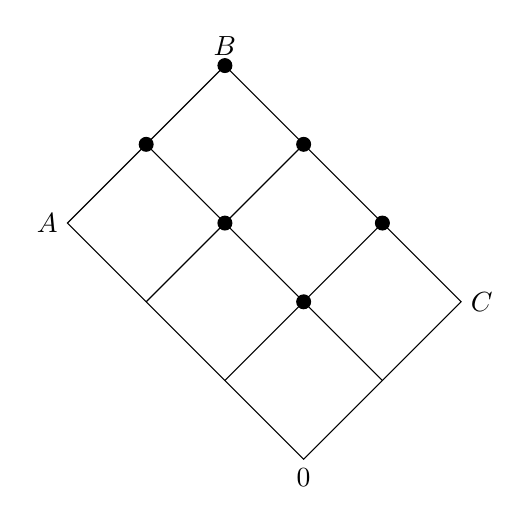
\begin{tikzpicture}[baseline={([yshift=-.5ex]current bounding box.center)}]
		\draw (-2,0) node[left] {$A$} -- (1,-3) node[below] {$0$}
		-- (3,-1) node[right] {$C$} -- (0,2) node[above] {$B$}-- cycle;
		\draw (-1,-1) -- (1,1);
		\draw (-1,1) -- (2,-2);
		\draw (0,-2) -- (2,0);
			\node[circle,draw=black, fill=black, inner sep=0pt,minimum size=5pt] at (1,1) {};
	\node[circle,draw=black, fill=black, inner sep=0pt,minimum size=5pt] at (0,2) {};
	\node[circle,draw=black, fill=black, inner sep=0pt,minimum size=5pt] at (-1,1) {};
	\node[circle,draw=black, fill=black, inner sep=0pt,minimum size=5pt] at (0,0) {};
	\node[circle,draw=black, fill=black, inner sep=0pt,minimum size=5pt] at (1,-1) {};
	\node[circle,draw=black, fill=black, inner sep=0pt,minimum size=5pt] at (2,0) {};
	\end{tikzpicture}
	\qquad \text{or}
	\qquad
	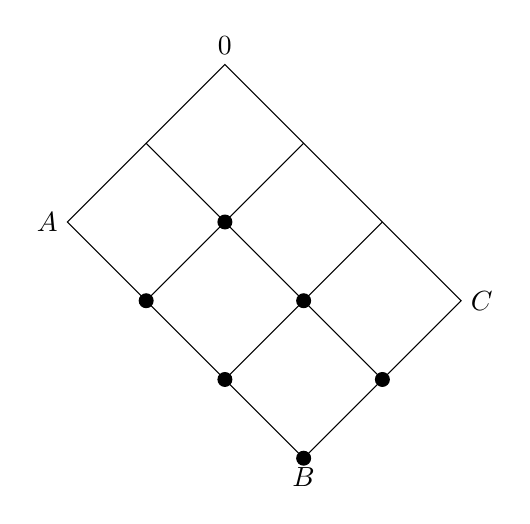
\begin{tikzpicture}[baseline={([yshift=-.5ex]current bounding box.center)}]
		\draw (-2,0) node[left] {$A$} -- (1,-3) node[below] {$B$}
		-- (3,-1) node[right] {$C$} -- (0,2) node[above] {$0$}-- cycle;
		\draw (-1,-1) -- (1,1);
		\draw (-1,1) -- (2,-2);
		\draw (0,-2) -- (2,0);
			\node[circle,draw=black, fill=black, inner sep=0pt,minimum size=5pt] at (0,0) {};
	\node[circle,draw=black, fill=black, inner sep=0pt,minimum size=5pt] at (1,-3) {};
	\node[circle,draw=black, fill=black, inner sep=0pt,minimum size=5pt] at (-1,-1) {};
	\node[circle,draw=black, fill=black, inner sep=0pt,minimum size=5pt] at (0,-2) {};
	\node[circle,draw=black, fill=black, inner sep=0pt,minimum size=5pt] at (2,-2) {};
	\node[circle,draw=black, fill=black, inner sep=0pt,minimum size=5pt] at (1,-1) {};
	\end{tikzpicture}
\end{center}
we can see that
\[
A+C-B=0.
\]
Since $A,B,C\geq 0$, the above equation forces $A$ and $C$ to vanish when $B=0$. Therefore, $B$ is no longer a facet of the degeneration. Similarly, black points are all vanishing facets in the above example, and generally
the number of vanishing facets equals the number of deleted $c$s for degenerations of this type.

One can use these diamonds to build a degeneration with more vanishing facets whose big polytope is a simplex. For example, in $A_3$
\begin{center}
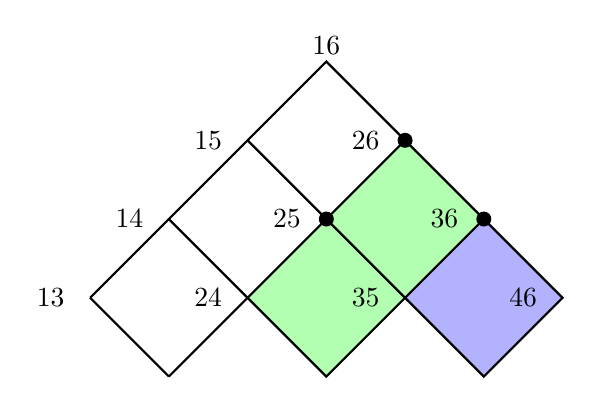
\begin{tikzpicture}
	\fill[green!30] (2,1) -- (0,-1) -- (1,-2) -- (3,0);
	\fill[blue!30] (3,0) -- (2,-1) -- (3,-2) -- (4,-1);
	\draw[thick] (-2,-1) -- (1,2) -- (4,-1) -- (3,-2) -- (0,1);
	\draw[thick] (-1,-2) -- (2,1);
	\draw[thick] (-2,-1) -- (-1,-2);
	\draw[thick] (-1,0) -- (1,-2) -- (3,0);
	\node[circle,draw=black, fill=black, inner sep=0pt,minimum size=5pt] at (1,0) {};
	\node[circle,draw=black, fill=black, inner sep=0pt,minimum size=5pt] at (2,1) {};
	\node[circle,draw=black, fill=black, inner sep=0pt,minimum size=5pt] at (3,0) {};
	\node at (-2.5,-1) {$13$};
\node at (-0.5,-1) {$24$};
\node at (1.5,-1) {$35$};
\node at (3.5,-1) {$46$};
\node at (-1.5,0) {$14$};
\node at (0.5,0) {$25$};
\node at (2.5,0) {$36$};
\node at (-0.5,1) {$15$};
\node at (1.5,1) {$26$};
\node at (1,2.2) {$16$};
\end{tikzpicture}
\end{center}
after setting $c$s in green and purple diamonds to be zero, three facets (black points) vanish and building set after deletion is 
\[
\{16,15,26,14,36,13,46\}.
\]
One can further check that it's a cube or $A_1^3$.

We can play the game for any degenerations of $A_n$, count black points and deleted $c$s in each degeneration, and find that for $A_2$, $A_3$ and $A_4$, there're respectively $5$, $42$ and $565$ possible degenerations whose big polytopes are simplices. For these degenerations, we can easily find their $u$-variables if their sets of all vanishing facets are known.

Suppose $\mathscr D$ is the set of all vanishing facets of a degeneration in the building set, 
we can read from the mesh that
\[
F_{I'}=\sum_{I\not\in \mathscr D}M_{I'}^IF_I
\]
for any $I'\in \mathscr D$, where $M$ is a matrix with non-negative entries. 
Therefore,
\[
\prod_{I\in \mathscr A_n}u_{I}^{F_{I}}=
\prod_{I'\in \mathscr D}u_{I'}^{F_{I'}}
\cdot
\prod_{I\not\in \mathscr D}u_{I}^{F_{I}}=
\prod_{I\not\in \mathscr D}\biggl(
u_I\prod_{I'\in \mathscr D}u_{I'}^{M_{I'}^I}
\bigg)^{F_I},
\]
so the new $u$-variables of the degeneration are
\[
    \tilde u_{I}=u_I\prod_{I'\in \mathscr D}u_{I'}^{M_{I'}^I}
\]
for any $I\not\in \mathscr D$. 

The simplest degenerations of $A_n$ are those with one $c_{i,i+2}$ vanishing. For the one with $c_{i,i+2}=0$, we get 
\[
F_{i,i+3}=F_{i,i+2}+F_{i+1,i+3},
\]
so 
\[
\tilde u_{i,i+2}=u_{i,i+2} u_{i,i+3},\quad 
\tilde u_{i+1,i+3}=u_{i+1,i+3} u_{i,i+3},\quad 
\tilde u_I=u_I \text{ for the other $I\neq (i,i+3)$}.
\]
They satisfy the following $u$-equation
\[
1-\tilde u_{i,i+2}=\prod_{j\neq i,i+2,i+3} \tilde u_{i+1,j},\quad 
1-\tilde u_{i+1,i+3}=\prod_{j\neq i,i+2,i+3} \tilde u_{i+2,j}
\]
and $u$-equations for $\{u_{kl}\,:\, (k,l)\neq (i,i+3),(i,i+2),(i+1,i+3)\}$ with the change of variables above. Similarly, one can easily find the $u$-variables and $u$-equations for the degenerations with $c_{i,i+2}=0$ for several $i$.

The next simplest degenerations of $A_n$ is setting $c_{i-1,i+1}=c_{i,i+2}=c_{i-1,i+2}=0$, we have seen an example in $A_3$ above.

% For example, in the above example of $A_3$,
% \[
% F_{123}=F_{1}+F_2+F_3, \quad F_{12}=F_1+F_2, \quad F_{23}=F_2+F_3,
% \]
% so the $u$-variables are
% \begin{align*}
% \tilde u_{1}&=u_1 u_{123} u_{12}=\frac{x_1}{x_{01}},\quad 
% \tilde u_{2}=u_2 u_{123} u_{12}u_{23}=\frac{x_{2}}{x_{012}},\quad 
% \tilde u_{3}=u_3u_{123}u_{23}=\frac{x_3}{x_{0123}},\\
% \tilde u_{0}&=u_{0}=\frac{x_{0}}{x_{01}},\quad 
% \tilde u_{01}=u_{01}=\frac{x_{01}}{x_{012}},\quad 
% \tilde u_{012}=u_{012}=\frac{x_{012}}{x_{0123}},
% \end{align*}
% and they satisfy the following $u$-equations:
% \[
% 	\tilde u_1+\tilde u_0=1,\quad \tilde u_2+\tilde u_{01}=1,
% 	\quad \tilde u_{3}+\tilde u_{012}=1.
% \]




(Find those with perfect $u$-eq?)

*******************
\subsection*{Degenerations which lead to products}
In this section we provide an answer to the question of which degenerations of $A_n$ and $B_n$ give the most general products of such geometries. We begin by stating the following results about Nestohedra.

The maximal set of a building set $B_{max}$ is the set of all inclusion maximal elements of the building set $B$. A building set $B$ is connected if $B_{max}$ has a single element.

{\bf Theorem:}If $B_1, B_2,\cdots B_n$ are connected subsets of a building set $B$ then the corresponding nestohedron ${\mathscr N_B}$ is isomorphic to the product of the nestohedra ${\mathscr N}_{ B_1} \times{\mathscr N}_{ B_2} \cdots \times {\mathscr N}_{B_n}$.

We can use the above result to construct 	a degeneration of $A_n$ which is a most general product i.e., $\prod_{p_i} A_{p_i}$ such that $\sum_{i} p_{i} = n$. 

Let us consider the  $A_4$ example for which the allowed possibilities are : $A_1^{4}$, $A_1^2 \times A_2$, $A_1 \times A_3$ and $A^{2}_2$.
 
For the $A_1^{4}$ the building set is $ \{ {0},{1},{2},{3},{4},{01},{12},{23},{34} \}$ where $\{0,01\} , \{1,12\},\{2,23\},\{3,34\}$ generate the 4 $A_1$'s.

For the $A_1^{2} \times A_2$ the building set is $ \{ {0},{1},{2},{3},{4},{01},{12},{23},{34},{234} \}$ where $\{0,01\} , \{1,12\} $ generate the 2 $A_1$'s and $\{2,3,4,23,34,234\}$ generates the $A_2$'s.

For the $A_1 \times A_3$ the building set is $ \{ {0},{1},{2},{3},{4},{01},{12},{23},{34},{123},{234},{1234} \}$ where $\{0,01\}$ is the generates the $A_1$ and $\{{1},{2},{3},{4},{12},{23},{34},{123},{234},{1234} \}$ generate  $A_3$'s.

For the $A_2^{2}$ the building set is $ \{ {0},{1},{2},{3},{4},{01},{12},{23},{34} ,{012},{234}\}$ where $\{0,1,2,01,12,012\}$  and $\{2,3,4,23,34,234\}$ generate the 2 $A_2$'s.

We can similarly find a degeneration of $A_n,B_n,~or~ {\mathscr P_n}$ which would correspond to any product.


\section{Stringy canonical forms and $u$-equations for generalized permutahedra}
In this section we shall argue that  a large subset of generalised permutahedra which are realised as degenerations of permutahderon ${\mathscr P_n}$ are binary geometries. Before we proceed we shall review some details about the generalised permutahedra which we shall use throughout the paper.
\subsection{Generalized permutohedra} 
A generalised permutahedron is a polytope that obtained as Minkowski sums and diffrences of co-ordinate simplices. 

Let, $\Delta_{[0,n]} = {\rm ConvexHull}(e_1,\cdots,e_n)$ be the standard coordinate simplex in $\mathbb{R}^{n+1}$. Then we have:
  \bea
{\mathscr P_n}^y(\{y_I \})= \sum y_I . \Delta_I  
 \eea
 for some collection of subsets $I \in [0,n]$
 We shall restrict ourselves to the large class of generalised permutahedra which admit such a realisation only as Minkowski sums i.e., all $y_I \ge 0$ \footnote{This is mainly due to the subtle nature of the Minkowski difference operation, which makes the shape of the resulting polytope dependent on the relative magnitudes of $y_I$'s.}which are called Nestohedra. Throughout the paper we shall mean Nestohedra whenever we refer to generalized permutahedra unless stated otherwise.\\
 
 The combinatorial structure of the generalised permutahedron ${\mathscr P_n({y_I})}$ (Nestohedra) is independent of the parameters $y_I$ and depends only on the collection of subsets $I \in [0,n]$ called the  building set ${\mathbf B}$.  
A collection of non-empty subsets of $[0,n]$ is called a building set ${\mathbf B}$ if it satisfies the following:
\begin{compactenum}[\quad (1)]
    \item If $I,J \in {\mathbf B}$ and $I \cap J \neq \phi $, then $I \cup J \in {\mathbf B}$.
    \item ${\mathbf B}$ contains all singletons $\{ i\}$ for $i \in S$.
\end{compactenum}
To describe the combinatorial structure we need the notion of {\it Nested complex} which we shall define now.

\subsubsection*{Nested Complex}
A subset ${\mathbf N}$ in the building set ${\mathbf B}$ is called a {\it nested set} if it satisfies the following conditions:
\begin{compactenum}[\quad (1)]
    \item For any $I,J \in {\mathbf N}$, we either have $I \subset J$ or $J\subset I$ or $I$ and $J$ are disjoint.
    \item For any collection of $k \geq 2$ disjoint subsets $J_1,J_2,\cdots, J_k \in N$ their union $J_1 \cup \cdots \cup J_k$ is not in B.
    \item ${\mathbf N}$ contains all maximal elements of $B$.
\end{compactenum}
The {\it nested complex} ${\mathbf N}({\mathbf B})$ is defined as the poset of the set of all nested sets in ${\mathbf B}$ ordered by inclusion.\\

 {\bf Facial structure:} 
 
 Let us assume that the set ${\mathbf B}$ associated with a generalised permutahedron ${\mathscr P_n}^{y}$ is a building set on $[0,n]$. Then the poset of faces ${\mathscr P_n}^{y}$ ordered by reverse inclusion is isomorphic to the nested complex ${\mathbf N}({\mathbf B})$. 

For each decomposition $[0,n]=  \sqcup_{I \subset {\mathbf N} } S_I $ where $S_I$ are non-empty, the face $P_n$ of ${\mathscr P_n}^{y}(y_I)$ associated with the nested set ${\mathbf N} \in {\mathbf N}({\mathbf B})$ is:
\bea
P_n = \sum_{{J \subset {\mathbf B}}\atop{J \cap S_I \neq \emptyset}} y_{J} \Delta_{J \cap S_I}
\eea

In summary the above results mean the following:\\

(1) We can look at any collection of subsets of $[0, n]$ which form a building set ${\mathbf B}$ and associate  coordinate simplex $\Delta_I$ for each $I \in {\mathbf B}$ and resulting Minkowski sum with positive weights $y_I$ generates a polytope of dimension $n$ called the generalised permutahedron (Nestohedron) associated with the building set. \\

(2) The number of facets $N$ of the generalised permutahedron just corresponds to the set of all elements in ${\mathbf B}$ excluding the maximal set. \\ 

(3) Two facets corresponding to the sets $I$ and $J$ in ${\mathbf B}$ intersect i.e., are {\it compatible} with each other if and only if  either $I \subset J$,~ $J \subset I$~ or $I \cap J = \emptyset ~{\text and} ~ I \cup J \notin {\mathbf B}$.

Let us look at a couple of examples to appreciate these facts better:\\
(1) Consider the generalized permutahedron with building set ${\mathbf B}= \{ \{0\},\{1\},\{2\},\{0,1\},\{1,2\},\{0,1,2\} \}$.

The polygon has 5 facets which correspond to the sets $\{ \{0\},\{1\},\{2\},\{0,1\},\{1,2\}\}$ and their compatability is shown in the figure below.

The polytope in this case is the 2d associahedron ${\mathscr A_2}$.\\
(2) Consider the generalized permutahedron with building set ${\mathbf B}= \{ \{0\},\{1\},\{2\},\{0,1\},\{1,2\},\{0,2\},\{0,1,2\} \}$ 

The polygon has 6 facets which correspond to the sets $\{ \{0\},\{1\},\{2\},\{0,1\},\{1,2\},\{0,2\}\}$ and their compatability is shown in the figure below.

The polytope in this case is the 2d cyclohedron ${\mathscr B_2}$ which also coincides with 2d permutahderon ${\mathscr P_2}$.
\begin{figure}[H]
\begin{center}       

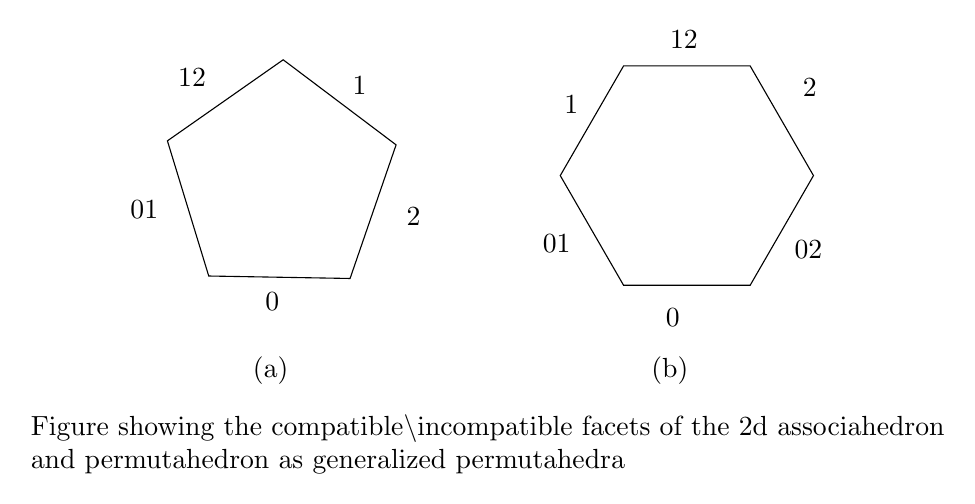
\begin{tikzpicture}[x=0.75pt,y=0.75pt,yscale=-1,xscale=1]
%uncomment if require: \path (0,511); %set diagram left start at 0, and has height of 511

%Shape: Regular Polygon [id:dp6636381249952382] 
\draw   (332.23,134.19) -- (310.06,198.57) -- (241.97,197.38) -- (222.06,132.26) -- (277.84,93.2) -- cycle ;
%Shape: Regular Polygon [id:dp8232688760864714] 
\draw   (533.33,149) -- (502.83,201.83) -- (441.83,201.83) -- (411.33,149) -- (441.83,96.17) -- (502.83,96.17) -- cycle ;

% Text Node
\draw (401.67,176.33) node [anchor=north west][inner sep=0.75pt]   [align=left] {01};
% Text Node
\draw (461,212) node [anchor=north west][inner sep=0.75pt]   [align=left] {0};
% Text Node
\draw (412,109) node [anchor=north west][inner sep=0.75pt]   [align=left] {1};
% Text Node
\draw (463,78) node [anchor=north west][inner sep=0.75pt]   [align=left] {12};
% Text Node
\draw (527,101) node [anchor=north west][inner sep=0.75pt]   [align=left] {2};
% Text Node
\draw (523,179) node [anchor=north west][inner sep=0.75pt]   [align=left] {02};
% Text Node
\draw (268,204) node [anchor=north west][inner sep=0.75pt]   [align=left] {0};
% Text Node
\draw (226,96) node [anchor=north west][inner sep=0.75pt]   [align=left] {12};
% Text Node
\draw (310,100) node [anchor=north west][inner sep=0.75pt]   [align=left] {1};
% Text Node
\draw (336,163) node [anchor=north west][inner sep=0.75pt]   [align=left] {2};
% Text Node
\draw (203,160) node [anchor=north west][inner sep=0.75pt]   [align=left] {01};
% Text Node
\draw (262,235) node [anchor=north west][inner sep=0.75pt]   [align=left] {(a)};
% Text Node
\draw (454,235) node [anchor=north west][inner sep=0.75pt]   [align=left] {(b)};
% Text Node
\draw (155,263) node [anchor=north west][inner sep=0.75pt]   [align=left] {Figure showing the compatible\textbackslash incompatible facets of the 2d associahedron  \\ and permutahedron as generalized permutahedra};


\end{tikzpicture}
\end{center}
\end{figure}
An improtant fact about generalised permutahedra which makes them particularly interesting is the following:
Let, $m$ denote the number of non-singlet elements in ${\mathbf B}$ i.e., the number of $c_J$'s as explained in equation (2) 
\bea
N &=& |{\mathbf B}|-1 \nonumber \\
 &=& (n+1+m)-1 \nonumber  \\
 &=& n+m \nonumber
\eea
{\bf Number of facets = Number of linear equations + dimension of  gen permutahedron}
 
Thus, generalised permutahedra have big Polytopes which are simplices. Thus its quite natural to wonder if the associated $u$-variables satisfy some kind of $u$-equations. 

We claim and we shall show in the next section that this indeed the case. Further we show that all these polytopes are binary geometries even though some of them do not admit perfect $u$-equations. 

Here are some interesting examples of generalised permutahedra:

(1) If ${\mathbf B}$ consists of only singlets i.e., ${\mathbf B}=\{ \{ 0,1,\cdots,n \}, \{ 0 \},\{ 1 \},\cdots ,\{ n \} \}$ then the generalised permutahedron is a Simplex. In this case the relevant $x$ variables are $x_i,~ i=0,\cdots,n$ with $x_0=1$ and $\sum_{i=0}^n x_i$. 
The Newton polytope of the Minkowski sum is $\prod_{i=1}^{n} x_i (1+\sum_{j=1}^{n} x_j)$ and $u$-variables are 
$u_i =\frac{ x_i}{1+\sum_{i=1}^n x_i} $
which satisfy $\sum u_i =1$ as their only $u$-equation. \\

(2) If ${\mathbf B}= \{[i] | i=1,\cdots,n+1 \}$ is the complete flag of intervals, then ${\mathscr P_n}^y({\bf Y})$ is the Stanley-Pitman polytope or Hypercube.
The Newton polytope of the Minkowski sum is $x_1\cdots x_n (1+x_1) \cdots (1+x_1+\cdots +x_n)$ and $u$-variables are 
$u_i =\frac{ 1}{1+\sum_{j=1}^{i} x_j} $, ~~$u^{'}_i =\frac{ \sum_{j=1}^{i} x_j}{1+\sum_{j=1}^{i} x_j} $ for $j=1,\cdots,n$ \\
which satisfy $u_i +u^{'}_{i} =1$ as their $u$-equation. \\

(3) If ${\mathbf B}$ corresponds to all the non empty subsets of $[0,n]$ and $Y_I =y_{|I|}$ i.e., the variables $Y_I$ are equal for all subsets of the same cardinality, then ${\mathscr P_n}({\bf Y})$ is the usual permutahedron ${\mathscr P_n}$. \\

(4)If ${\mathbf B}=\{ [i,j] | 1\leq  i \leq j \leq n\}$ is the set of consecutive intervals, then ${\mathscr P_n}({\bf Y})$ is the associahedron. \\

(5) If ${\mathbf B}=\{ [1,i] \cup [j,n] | 1\leq  i \leq j \leq n\}$ is the set of cyclic intervals, then ${\mathscr P_n}({\bf Y})$ is the Cyclohedron.\\

(6) Let $\Gamma$ be a graph on the vertex set $[0,n]$. Let us assume that ${\mathbf B} = {\mathbf B}(\Gamma)$ is the set of subsets $I \in [n]$ such that the induced graph $\Gamma$ is connected, then  ${\mathscr P_n}({\bf Y})$ is a graph associahedron.

It is clear that any  generalized permutahedron can be obtained as a degeneration of  permutahedron ${\mathscr P_n}$i.e., by removing some elements from its building set. This makes the permutahedron a very important example of generalized permutahedra and we shall devote the rest of this section to studying its properties and proving it is binary.
\subsubsection*{Permutahedron}

Let, $\Delta_{[0,n]} = {\rm ConvexHull}(e_1,\cdots,e_{n+1})$ be the standard coordinate simplex in $\mathbb{R}^{n+1}$. For any $I \subset [0,n] $ let $\Delta_I ={\rm ConvexHull}(e_i~|~i\in I)$ denote the face of the $\Delta_{[0,n]}$. The polytope $P_n(\{y_I \})$ obtained as the Minkowski sum of simplices $\Delta_I$ scaled by  parameters $y_I > 0$ for all nonempty subsets $I \subset [n+1]$
 \bea
 P_n(\{y_I \})= \sum_{I \subset[n+1]} y_I . \Delta_I  
 \eea
 is the permutahedron ${\mathscr P_n}$

{\bf Facial Structure:} 

The $(n-k)$ faces of ${\mathscr P_n}$ are in an $1-1$ correspondence with the decomposition of $[0,n]$ into $k$ parts. More precisely, for each $(S_1,\cdots,S_k)$ with $S_i \neq \emptyset ~ \forall i$ and $[0,n] = S_1 \sqcup \cdots \sqcup S_k$ the corresponding face $\pi_{S_1,\cdots,S_k}$ has vertices which are permutations such that the entries $ \{x_i | i \in S_1 \}$ are largest $|S_1|$ numbers in $[0,n]$, $\{x_i | i \in S_2 \}$ are largest $|S_2|$ numbers in $[0,n]$ and so on. 

Further the face $\pi_{S_1,\cdots,S_k}$   is isomorphic to ${\mathscr P_{\left(| S_1|-1\right)} }\times {\mathscr P_{\left(| S_2|-1\right)} } \cdots \times{\mathscr P_{\left(| S_k|-1\right)} } $.

It follows from above that ${\mathscr P_n}$ has $2^{n+1} -2$ facets corresponding to all the non-empty proper subsets of $[0,n]$ for which we have a decomposition $[0,n] = S \sqcup S^c$ and the facets are isomorphic to one of the following product of lower dimensional permutahedra  $ \{ {\mathscr P_{n-1}}, {\mathscr P_{n-2}} \times A_1, \cdots ,{\mathscr P_{\lfloor{n/2 \rfloor}}} \times {\mathscr P_{n-1-\lfloor n/2 \rfloor}}  \} $\footnote {More generally the number of $(n-k)$ facets of ${\mathscr P_n}$ is $ k! S(n,k)$ where $S(n,k)$ is the Stirling number of the second kind which counts the number $k$ partitions of  $I$ and there are $p(n+1,k)$ types where $p(n+1,k)$ is the number of $k$ partitions of $(n+1)$.}.

It also follows from above that a face $\pi_{S_1,\cdots,S_k}$ is contained in another face $\pi_{T_1,\cdots,T_l}$ if and only if each $T_i$ is a union of consecutive $S_j$ or equivalently if $(S_1,\cdots,S_k)$ is a refinement of $(T_1,\cdots,T_l)$.

\section*{ABHY like realisation for the Permutahedron}
The following set of equations to define the $n$-dimensional Permutahedron: 
\bea
C_I = (-1)^{|I|} \left( \sum_{i \in I} X_i - \sum _{{i<j}\atop{i,j \in I}} X_{ij} +\cdots + (-1)^{|I|}  X_I \right) \nonumber
\eea
for all non-empty subsets $I \subset \{0,1,\cdots,n\}$ with the understanding that $C_{I} =0$ for all singlets $I$ and $X_{I} =0$ for $I=\{ 0,1,\cdots,n \}$. 

It is clear that
\bea
m= \text{No. of  C's }&=& 2^{n+1}-(n+2) \nonumber \\
N= \text{No. of X's} &=& 2^{n+1}- 2 \nonumber 
\eea
Thus we see that $N= d+m$ as expected. We can write down the stringy integral as usual to be 
\bea
\int_{\mathbb{R}^{n}_{+}} \prod_{i =1}^{n} d x_i x_i^{\alpha^{'} X_i -1} \prod_{I} \left (\sum_{a\in I} x_a \right) ^{-\alpha^{'} C_I} \nonumber
\eea 
where the product is over all non-singlets $ I \subset \{0,1,\cdots,n\}$ with $x_{0} =1$.

Let us look at the $n=2,3$ examples:

\section*{2d permutahedron}
In this case the building set $B=\{ \{ 0,1,2\},\{ 0,1\},\{0,2\},\{1,2\},\{0\},\{1\},\{2\}\}$ and the relevant $x$ variables are $x_0=1, ~x_1=x, ~x_2=y, ~x_{01}=1+x, ~x_{02}=1+y,~ x_{12}=x+y,~ x_{012}=1+x+y$. 

We can write down the Newton polynomial for the Minkowski sum as $ x_1~ x_2~(1+x_1)~(1+x_2)~(x_1+x_2)~(1+x_1+x_2)$.

The $u$-variables can be written in terms of $x$ variables as:
\bea
u_1&=&\frac{x(1+x+y)}{(x+y)(1+x)}, ~ u_2 =\frac{y(1+x+y)}{(x+y)(1+y)},~ u_{12}=\frac{(x+y)}{(1+x+y)}\nonumber \\
u^{'}_1&=&\frac{(1+y)}{(1+x+y)}, ~~~~~ u^{'}_2=\frac{(1+x)}{(1+x+y)},~~~~~ u^{'}_{12}= \frac{(1+x+y)}{(1+x)(1+y)} \nonumber
\eea
The $u$-equations are:
\bea
1-u_i &=& (u^{'}_i)^2 u_j u^{'}_{12}, ~~~ 1-u_{12} = u^{'}_{1} u^{'}_{2} u^{'}_{12} \nonumber \\
1-u^{'}_i &=& u_i u^{'}_j u_{12}, ~~~~~~~ 1-u^{'}_{12} = u_{1} u_{2} (u_{12})^2 \nonumber
\eea
where $i=1$ implies $j=2$ and vice versa.

\section*{3d permutahedron}
In this case the building set $B=\{ \{ 0,1,2,3\},\{ 0,1,2\},\{0,2,3\},\{0,1,3\},\{1,2,3\},\{0,1\},\{0,2\},\{0,3\},\{1,2\} \\ ,\{2,3\},\{1,3\},\{0\},\{1\},\{2\},\{3\}\}$ and the relevant $x$ variables are $x_0=1, ~x_1=x, ~x_2=y, ~x_3=z, ~x_{01}=1+x, ~x_{02}=1+y,~x_{03}=1+z,~ x_{12}=x+y,~x_{13}=x+z,~x_{23}=y+z,~ x_{012}=1+x+y,~ x_{013}=1+x+z,~ x_{023}=1+y+z,~ x_{123}=x+y+z,~ x_{0123}=1+x+y+z$. \\

The $u$ and $u'$-variables can be written interms of $x$ variables as:
{\scriptsize  \bea
u_1&=&\frac{x(1+x+y)(1+x+z)(x+y+z)}{(x+y)(x+z)(1+x)(1+x+y+z)}, ~ u_2 =\frac{y(1+x+y)(1+y+z)(x+y+z)}{(x+y)(y+z)(1+y)(1+x+y+z)},~ u_{3}=\frac{z(1+x+z)(1+y+z)(x+y+z)}{(x+z)(y+z)(1+z)(1+x+y+z)},\nonumber \\
u^{'}_1&=&\frac{(1+y+z)}{(1+x+y+z)}, ~~~~~~~~~~~~~~~~~~~~~~~~~~~~ u^{'}_2 =\frac{(1+x+z)}{(1+x+y+z)},~~~~~~~~~~~~~~~~~~~~~~~~~~~~~ u^{'}_{3}=\frac{(1+x+y)}{(1+x+y+z)},\nonumber \\
u_{12}&=&\frac{(x+y)(1+x+y+z)}{(1+x+y)(x+y+z)}, ~~~~~~~~~~~~~~~~~~ u_{23} =\frac{(y+z)(1+x+y+z)}{(1+y+z)(x+y+z)},~~~~~~~~~~~~~~~~~~~ u_{13}=\frac{(x+z)(1+x+y+z)}{(1+x+z)(x+y+z)},\nonumber \\
u^{'}_{12}&=&\frac{(1+z)(1+x+y+z)}{(1+y+z)(1+x+z)}, ~~~~~~~~~~~~~~~~~~ u^{'}_{23} =\frac{(1+x)(1+x+y+z)}{(1+x+y)(1+x+z)},~~~~~~~~~~~~~~~~~~~ u^{'}_{13}=\frac{(1+y)(1+x+y+z)}{(1+x+y))(1+y+z)},\nonumber  \\
u_{123}&=&\frac{(x+y+z)}{(1+x+y+z)}, ~~~~~~~~~~~~~~~~~~~~~~~~~~~ u^{'}_{123} =\frac{(1+x+y)(1+y+z)}{(1+x)(1+y)(1+z)(1+x+y+z)}\nonumber
\eea }
The $u$-equations in this case are:
{\small  \bea
1-u_i &=& u_j u_k (u_{jk})^2 (u^{'}_i)^3 (u^{'}_{ij})^2(u^{'}_{ik})^2 u^{'}_{123} \left(1+ u_i u_{ij} u_{ik} u^{'}_{j} u^{'}_{k}  u^{'}_{jk}\right), ~~ 1-u_{ij} = u_k u_{ik} u_{jk} (u^{'}_i)^2 (u^{'}_{j})^2 (u^{'}_{ij})^2 u^{'}_{ik} u^{'}_{jk} u^{'}_{123} \nonumber  \\
1-u^{'}_i &=& u_i u_{ij} u_{ik} u^{'}_{j} u^{'}_{k}  u^{'}_{jk}, ~~~~~~~~~~~~~~~~~~~~~~~~~~~~~~~~~~~~~~~~~~~~~~~~~~~~~ 1-u^{'}_{ij} = u_i u_{j}  (u_{ij})^2 u_{ik} u_{jk} (u_{123})^2 (u^{'}_{k})^2 u^{'}_{ik} u^{'}_{jk}  \nonumber \\
1-u^{'}_{123} &=& u_1 u_{2} u_{3} (u_{12})^2 (u_{23})^2  (u_{13})^2 (u_{123})^3 \left(1+ u^{'}_{123}  u^{'}_1 u^{'}_{2} u^{'}_{3} u^{'}_{12} u^{'}_{23}  u^{'}_{13} \right), 1-u_{123} = u^{'}_1 u^{'}_{2} u^{'}_{3} u^{'}_{12} u^{'}_{23}  u^{'}_{13} u^{'}_{123}   \nonumber
\eea}
where $i,j,k \in {1,2,3}$ and $i \neq j \neq k$.

The 8 facets of the 3d permutahedron corresponding to $u_i \rightarrow 0, u^{'}_i \rightarrow 0,u_{123} \rightarrow 0 ~and ~u^{'}_{123} \rightarrow 0$  are all $B_2$'s. Similarly, the 6 facets corresponding to  $u_{ij} \rightarrow 0, u^{'}_{ij} \rightarrow 0$ are all  $A^{2}_1$.

Thus, the 3d permutahedron integral factorizes nicely on all massless poles at finite $\alpha^{'}$ !!
We shall list a few results about permutahedra which shall be useful for later purposes: 
\begin{enumerate}
\item The $u$-variables for the permutahedron are: 
\bea
u_J &=& ~~\prod_{J \subset I} x_I^{(-1)^{|I|-|J|}} \nonumber 
\eea
The above relations can also be inverted to obtain $x_I$ as follows:

For $0 \notin I $
\bea
x_I &=& \frac{\prod_{I \subset J} u_{J}}{1-\prod_{I \subset J} u_{J}} \\
\frac{1}{1+ x_I} &=& \prod_{{J}\atop{J\cap \bar{I} \ne \emptyset}} u_{\bar{J}}
\eea
From the above relations it is clear that taking $u_I \rightarrow 0$ for $0 \notin I$ implies $x_J \rightarrow 0$ for all $J \subset I$ and taking $u_{\bar{I}} \rightarrow 0$ implies $x_J \rightarrow \infty $ for all $I \subset J$.
In fact we shall argue that there is unique choice of $x_I$'s which we can take to $0$ or $\infty$ which corresponds to setting only a particular $u_I \rightarrow 0$ or $u_{\bar{I}} \rightarrow 0$ respectively.
\item From the definition of the permutahedron as a Nestohedron we know that $I$ and $J$ are :

% {\bf compatible if} $I\cap J = \emptyset$ or $I\cap J \neq \emptyset$ and either $I \subset J$ or $J \subset I$

% {\bf incompatible if}   $I\cap J \neq \emptyset$ or $I\cap J = \emptyset$ and neither $I \not\subset J$ or $J \not\subset I$

{\bf compatible if and only if} $\{[0,n],I,J\}$ is a nested set, i.e.
\[
I\subset J\quad \text{or}\quad J\subset I\quad \text{or}\quad (J\cap I=\varnothing \quad \text{and}\quad J\cup I\not\in \mathscr P_n).
\]
For permutohedron, $J\cup I$ is always contained in $\mathscr P_n$ for any $I$ and $J$, so it's compatible if and only if $J\subset I$ or $I\subset J$.

The above  follows directly from the following relations amongst $u$ for each $I$ such that $0\notin I$ :
\bea
1-\prod_{I \subset J} u_{J} &=& \prod_{{J}\atop{J\cap \bar{I} \ne \emptyset}} u_{\bar{J}} \\
1-\prod_{J \subset I} u_{\bar{J}} &=& \prod_{I \subset J} u_{J} \prod_{J \subset \bar{I} } u_{\bar{J}}
\eea


\section*{Braid arrangement}
The braid arrangement in $\mathbb{R}^{n+1}$ consists of $\left({n}\atop{2}\right)$ hyperplanes 
\bea
z_i =z_j ~~{\rm for ~ all}~~0 \leq i<j \leq n
\eea 
\subsection{Natural stringy integrals with linear factors} 

{\bf introduce a natural stringy integrals for any generalized stringy canonical forms: variables $x_0=1, x_1, \cdots, x_n$ and define $x_I=\sum_{i \in I} x_i$, the factors are $x_I^{\alpha' S_I}$ (we can say monomials $S_\{i\}=X_i$ and polynomials $S_I=-c_I$. $N=n+m$ and big polytope is a simplex, then general formula for $u$ variables, which is equivalent to ABHY conditions; again $P_n$ in full details and others as degenerations.}

*******************

In the last subsection, we have seen that any $n$-dimensional generalized 
permutahedron can be constructed by a Minkowski sum of some simplices labeled by
subsets of $[0,n]$. For a simplex labeled by a subset $I$, 
it is natrual to associate the linear polynomial $x_I=\sum_{i\in I}x_i$ whose Newton polytope is the corresponding simplex. Therefore, we can write down a natrual stringy canonical form for the generalized permutahedron with the building set 
$\mathscr P$
\begin{equation} \label{stringyintforgenpermutohedron}
   \mathcal I_{\mathscr P}(\{S_I\})=\int_{\mathbb R^{n}_+}
	\frac{\prod_{i=0}^n \mathrm{d}\log x_i}
	{\operatorname{GL}(1)_+}\prod_{I\in\mathscr P}x_I^{\alpha' S_I},
\end{equation}
where the global $\operatorname{GL}(1)_+$ redundance $x_i\mapsto a x_i$ require that 
$\sum_{I\in\mathscr P}S_I = 0$. 

Generally, we can consider an arbitrary set of subsets of $[0,n]$ in eq.\eqref{stringyintforgenpermutohedron}. 
However, the big polytope for such integral in general is not a simplex.
It's highly non-trivial to figure out all such sets whose big polytopes are simplices,
but we can easily see that every generalized permutahedron satisfies $N=n+m$
because each facet $F_I$ is given by a nested set $\{[0,n],I\}$ for $I\neq [0,n]$.
Therefore, for a generalized permutahedron $\mathscr P$, we can write down the matrix 
$W^J_A$ of facets and then get $S_J=F_A(W^{-1})^A_J\geq 0$ and 
its $u$-variables $u_A=\prod_J p_J^{(W^{-1})^A_J}$.

Let's first write down equations of facets of a generalised permutahedron
with the building set $\mathscr P$. The polytope of 
eq.\eqref{stringyintforgenpermutohedron} is given by the Minkowski sum
\[
	- \sum_{I\in\mathscr P,|I|>1}S_I.\Delta_I
\]
in $(S_0,\dots,S_n)$-space, where $\Delta_I=\operatorname{ConvexHull}
(\{e_i\}_{i\in I})$. Meanwhile, we know from the last subsection that the facet 
labeled by a nested set $\{[0,n],I\}$ is given by
\begin{align*}
	\biggl\{(S_0,S_1,\dots,S_n)\in \mathbb R^{n+1}\,\bigg |\,
		\sum_{i\in I}S_i = -\sum_{J\subset I,|J|>1,J\in \mathscr P}S_J,
		\quad
		&\sum_{i=0}^nS_i=-\sum_{J\in \mathscr P,|J|>1}S_J,\\
		&\sum_{i\in K}S_i\geq -\sum_{J\subset I,|J|>1,J\in \mathscr P}S_J
	\biggr\},
\end{align*}
where the second constrain is just $\sum_{I\in \mathscr P}S_I=0$, so the equation 
of this facet is 
\begin{equation}\label{GPfacet}
	F_I:=\sum_{J\subset I,J\in\mathscr P}S_J=0.
\end{equation}

Within all generalized permutahedra, the original permutahedron is quite simple
and important because any other generalized permutahedron can be degenerated from
permutahedron by setting some $S_I$ to be zero.
The building set of the $n$-dimensional permutahedron $\mathscr P_n$ is 
the set of all non-empty subsets of $[0,n]$. 
To get $u$-equations, we should solve $S_J$ by $F_J$ from eq.\eqref{GPfacet}, the 
solution for permutahedron $\mathscr P_n$ is 
\begin{equation}\label{SinF}
	S_I=\sum_{J\neq \varnothing,J\subset I} (-1)^{|J|-|I|}F_J,
\end{equation}
then
\[
	\prod_{I\neq \varnothing,I\subset [0,n]}u_I^{F_I}=
	\prod_{I\neq \varnothing,I\subset [0,n]}x_I^{S_I}=
	\prod_{\varnothing\neq J\subset I\subset [0,n]}
	x_I^{(-1)^{|J|-|I|}F_J}=
	\prod_{J\neq \varnothing,J\subset [0,n]}
	\prod_{I\supset J}(x_I^{(-1)^{|J|-|I|}})^{F_J}
\]
gives that
\[
	u_I=\prod_{J\supset I}x_J^{(-1)^{|I|-|J|}}.
\]
For example, the $u$-variables of $\mathscr P_2$ are
\[
	u_{0}  = \frac{x_0 x_{012}}{x_{01}x_{02}},\quad 
	u_{1}  = \frac{x_1 x_{012}}{x_{01}x_{12}},\quad
	u_{2}  = \frac{x_2 x_{012}}{x_{02}x_{12}},\quad
	u_{01} = \frac{x_{01}}{x_{012}},\quad 
	u_{02} = \frac{x_{02}}{x_{012}},\quad
	u_{12} = \frac{x_{12}}{x_{012}}.
\]
They satisfy the following equations
\begin{align*}
	&1-u_{0}=u_{1} u_{2} u_{12}^2,
	1-u_{1}=u_{0} u_{2} u_{02}^2,
	1-u_{2}=u_{0} u_{1} u_{01}^2,\\
	&1-u_{01}=u_{2} u_{02} u_{12},
	1-u_{02}=u_{1} u_{01} u_{12},
	1-u_{12}=u_{0} u_{01} u_{02}.
\end{align*}
We will discuss these $u$-equations in the next subsection.

For permutahedra, we can give a ABHY construction from eq.\eqref{SinF} by setting 
$S_I=-c_I$ for any non-singleton $I\in \mathscr P_n$, where $c_I$ are positive 
constants, and a ABHY polytope is given by 
\begin{equation}\label{ABHY}
	F_I\geq 0,\quad -c_I=\sum_{J\neq \varnothing,J\subset I}(-1)^{|J|-|I|}F_J
\end{equation}
in $\{S_i=F_i\,:\,1\leq i\leq n\}$-space, where the last equation is a gauge fixing. 
According to eq.\eqref{genperm_defi}, this polytope is a $n$-dimensional 
permutahedron $\mathscr P_n$. {\bf (???)}
The ABHY construction of any generalized permutohedra can be obtained by 
setting $c_I=0$ for all $I$ not in the building set.

For example, the building set of $\mathscr A_2$ is $\mathscr P_2-\{\{0,2\}\}$,
its ABHY construction can be obtained from $\mathscr P_2$ by setting $c_{02}=0$, 
\[
	0=-c_{02}=F_{02}-F_2,
\]
therefore the whole ABHY conditions for $\mathscr A_2$ is 
\[
	-c_{01}=F_{01}-F_0-F_1,\quad -c_{12}=F_{12}-F_1-F_2,\quad 
	-c_{012}=-F_{01}-F_{12}+F_1,\quad F_I\geq 0,
\]
and its solution in $(F_1,F_2)$ space is 
\[
	\left\{\begin{aligned}
		F_1&\geq 0,F_2\geq 0\\
		F_0&=c_{01}+c_{12}+c_{012}-F_1-F_2\geq 0,\\
		F_{12}&=F_1+F_2-c_{12}\geq 0,\\
		F_{01}&=c_{012}+c_{12}-F_2\geq 0.
	\end{aligned}\right.
\]

\subsection{Binary geometries and $u$ equations}

% {\bf argue in general to have binary geometries we must have $1-u=\prod u' p(\{u\})$ with $p(u=0)=1$, conjecture that this is true of ALL gen. perm. Show it for gen. perm. more examples?}

\subsubsection{The binary aspects of $u$-variables for permutohedra}

Here we will show that the $u_{I}$'s for the permutahderon $\mathscr{P}_{n}$, which is defined as 
\begin{equation}
   u_{I}:= \prod_{J\supset I}x_J^{(-1)^{|I|-|J|}} \:, \label{uforpn}
\end{equation}
have the desired binary property, that is, $u_{I}$ and $u_{J}$ are compatible if and only if $I \subset J$ or $J\subset I$, otherwise, they are incompatible. Forthermore, we will show that the $u$-variables compatible with $u_{I}$ will become the $u$-variables for the facet $\mathscr{P}_{\lvert I \rvert-1}\times \mathscr{P}_{n-\lvert I\rvert}$ as $u_{I}$ gose to 0.
% In other words, this means that $u_{I}$ and $u_{J}$ are incompatible if $I$ and $J$ are one of the following two cases:
% \begin{enumerate}[resume]
%    \item $I\cap J=\emptyset$ and $I\cup J \in \mathcal{B}$ \:, 
%    \item $I\cap J \neq \emptyset,I, J $ \:.
% \end{enumerate}

A crucial observation here is that $u_{I}\to 0$ is equivalent to $x_{I}\to 0 $ according to \eqref{uforpn} since all $x_{i}$ are positive. We can approach this limit by replacing $x_{i}$ with $ \epsilon x_{i}$ for all $i\in I$ then taking $\epsilon \to 0$. Then the remaining task is just to consider the behaviour of the other $u_{J}$'s under this limit. 
% In the following arrangement, it is convenient to introduce 
% \begin{equation}
%   p(J_{1},J_{2},\cdots,J_{n}):= \sum_{j\in J } x_{j} \:.
% \end{equation}
% where $J= \bigcup_{a=1}^{n} J_{a}$

Let us first show that the $u$-variables incompatible with $u_{I}$ become 1 as $u_{I}$ goes to 0. It is obvious that $u_{I}$ and $u_{J}$ are incompatible if either (1) $I\cap J=  \varnothing$  or (2) $I\cap J \neq \varnothing,I, J $. For the first case, let us denote $K=[0,n]-(I\cup J)$ as the complement set of $[0,n]$ with respect to $I\cup J$. Then we find the logarithm of $u_{J}$ can be written as 
\begin{equation}
     \log u_{J} = \sum_{\kappa\subset K,\psi\subset I} (-1)^{\lvert\kappa\rvert+\lvert \psi\rvert }\log (x_{J}+x_{ \kappa} +x_{ \psi} )\:. \label{1incompuvarforPn}
\end{equation}
As $x_{i}\to 0$ with $i\in I$, we have 
\begin{equation}
   \log u_{J} \to \sum_{\kappa\subset K} (-1)^{\lvert \kappa\rvert } \log (x_{J}+x_{ \kappa})\Biggl(\sum_{\psi\subset I}(-1)^{\lvert\psi\rvert}\binom{\lvert \psi \rvert }{\lvert I \rvert }\Biggr)=0 \label{incompn1}
\end{equation}
where the binomial expansion of $(1-1)^{\lvert I \rvert}$ has been used. For the second case, the logarithm of $u_{J}$ can be written as 
\begin{equation}
   \log u_{J} = \sum_{\psi'\subset I',\kappa\subset K}(-1)^{\lvert \psi' \rvert+ \lvert \kappa\rvert}  \log (x_{J'}+ x_{(I\cap J)}+x_{ \psi'}+x_{\kappa })
\end{equation}
where $I'=I-J$, $J'=J-I$ and $K=[0,n]-(I\cup J)$. Then a similar argument as in \eqref{incompn1} gives $\log u_{J}\to 0$ under the limits of all $x_{i}\to 0$ with $i\in I$.

Now let us consider the behaviour of compatible $u$-variables under this limit. For $J\subset I$, we again introduce $I'=I-J$ and $K=[0,n]-I$, then the logarithm of $u_{J}$ can be written as 
\begin{equation}
     \log u_{J}=\sum_{\psi'\subset I', \kappa \subset K} (-1)^{\lvert \psi'\rvert +\lvert \kappa \rvert} \log (x_{J}+x_{\psi'}+x_{\kappa})
\end{equation}
Next, we replac $x_{i}$ with $ \epsilon x_{i}$ for all $i\in I$ and take $\epsilon \to 0$, then 
\begin{align}
   \log u_{J} &\to \lim_{\epsilon \to 0} \sum_{\psi'\subset I', \kappa \subset K} (-1)^{\lvert \psi'\rvert +\lvert \kappa \rvert} \log (\epsilon x_{J}+ \epsilon x_{\psi'}+x_{\kappa}) \nonumber  \\
    &=\lim_{\epsilon\to 0} \biggl(\log \epsilon+\sum_{\kappa\subset K,\kappa \neq \varnothing}\log x_{\kappa}\biggr)\Biggr( \sum_{\psi'\subset I'}(-1)^{\lvert\psi'\rvert}\binom{\lvert \psi' \rvert }{\lvert I \rvert }\Biggr)
    +\sum_{\psi'\subset I'} (-1)^{\lvert \psi'\rvert }\log (x_{J}+x_{\psi'}) \nonumber \\
    &=\sum_{\psi'\subset I'} (-1)^{\lvert \psi'\rvert }\log (x_{J}+x_{\psi'}) \label{subP1}
\end{align}
Obviously, the expression in the last line of \eqref{subP1} is exactly the $u$-variable for the permutahderon $\mathscr{P}_{\lvert I\rvert -1}$. For $J\supset I$, under the limit of $x_I\to 0$, the logarithm of $u_{J}$ simply becomes 
\begin{equation}
   \log u_{J} = \sum_{\kappa \subset K} (-1)^{\kappa} \log (x_{I}+x_{J-I}+x_{\kappa}) 
   \to  \sum_{\kappa \subset K} (-1)^{\kappa} \log (x_{J-I}+x_{\kappa}) 
\end{equation}
where $K=[0,n]-J$, which is exactly the $u$-variable for the permutahderon $\mathscr{P}_{n-\lvert I\rvert}$


\subsubsection{The binary aspects of $u$-variables for generalized permutohedra}

Inspired by the $u$-variables for permutahdera, we come up with the $u$-variables for generalized permutohedra. To this end, let us define the generating set $\mathbf{I}$ for $I\in\mathbf{B}$ as the set of the minimum extensions of $I$ on $\mathbf{B}$, that is there is no $J\in\mathbf{B}$ such that $I\subsetneq J\subsetneq I_{a}$ for any $I_{a}\in \mathbf{I}$. Then, the $u$-variables for the generalized permutohedron with building set $\mathbf{B}$ are 
\begin{equation}
   \log u_{I} :=  \log x_{I}- \sum_{I_{a}\in \mathbf{I}} \log x_{I_{a}}+\cdots +(-1)^{k}\sum _{I_{a_{1}},\cdots,I_{a_{k}}\in \mathbf{I}} \log x_{I_{a_{1}}\cup\cdots \cup I_{a_{k}}} +\cdots \:. \label{uvarforgenpermu}
\end{equation}
It is easy to check that the $u$-variables for associahedra, cyclohedra and permutohedra defined above can be viewed as the special cases of \eqref{uvarforgenpermu}. Let us give another slight nontrivial example to illustrate this defination.

\paragraph{Example:} For the generalized permutahderon with building set 
\[
\mathbf{B}=\{\{0\},\{1\},\{2\},\{3\},\{0,1,2\},\{1,3\},\{0,1,2,3\}\},
\]
the corresponding $u$-variables are
\begin{gather*}
   u_{0}=\frac{x_{0}}{x_{012}} \:,\quad  u_{1}=\frac{x_{1}x_{0123}}{x_{012}x_{13}} \:,\quad 
   u_{2}=\frac{x_{2}}{x_{012}} \:, \quad u_{3}=\frac{x_{3}}{x_{13}} \\
   u_{012}=\frac{x_{012}}{x_{0123}}\:,\qquad u_{13}=\frac{x_{13}}{x_{0123}} \:, \quad 
\end{gather*}

For generalized permutahdera, $u_{I}$ and $u_{J}$ are incompatible if $I$ and $J$ are one of the following two cases:
\begin{enumerate}
   \item $I\cap J=\varnothing$ and $I\cup J \in \mathbf{B}$ \:, 
   \item $I\cap J \neq \varnothing,I, J $ \:,
\end{enumerate}
while $u_{I}$ and $u_{J}$ are compatible if $I$ and $J$ are one of the following three cases:
\begin{enumerate}[resume]
   \item $J\subset I$\:,
   \item $I\subset J$ \:,
   \item $I\cap J=\varnothing$ and $I\cup J \notin \mathbf{B}$ \:.
\end{enumerate}
We will follow the argument in the cases of permutahdera: replacing $x_{i}$ with $ \epsilon x_{i}$ for all $i\in I$ and taking $\epsilon \to 0$, then considering the behaviour of the other $u_{J}$'s under this limit case by case. For future convenience, we assume that the generating set $\mathbf{J}$ for $J$ has $s$ elements denoted by $J_{a}$ with $a\in[1,s]$, and introduce 
\begin{equation}
   p(J_{1},\ldots,J_{r}) = \sum_{a\in J_{1}\cup\cdots\cup J_{r}}x_{a}
\end{equation}

For case (1), some elements in $\mathbf{J}$ are subsets of $I\cup J$ since $I\cup J \in \mathbf{B}$ (an extreme case is that  $I\cup J$ is one element in $\mathbf{J}$, but the argument is the same). Without loss of generality, we denote such elements by $J_{1},\ldots J_{s'}$. Then the logarithm of $u_{J}$ can be written as 
\begin{equation}
   \log u_{J}= \sum_{\substack {1 \leq a_{1}<\cdots<a_{k}\leq s'\\ s'<b_{1}<\cdots b_{l}\leq s}}(-1)^{k+l}\log\Bigl( x_{J}+ p(J_{a_{1}}-J,\ldots,J_{a_{k}}-J) + p(J_{b_{1}}-J,\ldots, J_{b_{l}}-J)\Bigr) \:. \label{logu1}
\end{equation}
Since the second term in eq.\eqref{logu1} goes to 0 under the limits of $x_{i}\to 0$ with $i\in I$, $\log u_{J}$ goes to 0 under this limit as in eq.\eqref{1incompuvarforPn}. The whole argument can be carried over to case (2) by replacing $x_{J}$ with $x_{I\cap J}+ x_{J-I}$.

For case (3), we again denote $J_{1},\ldots J_{s'}$ as the elements in $\mathbf{J}$ which are subsets of $ I$. After replacing $x_{i}$ with $\epsilon x_{i}$ for $i\in I$, we find the limit of $\log u_{J}$ as $\epsilon \to 0$ is
\begin{align}
  &\quad \lim_{\epsilon\to 0}  \sum_{\substack {1 \leq a_{1}<\cdots<a_{k}\leq s'\\ s'<b_{1}<\cdots b_{l}\leq s}}(-1)^{k+l}\log\Bigl( \epsilon x_{J}+\epsilon p(J_{a_{1}}-J,\ldots,J_{a_{k}}-J) + p(J_{b_{1}}-J,\ldots, J_{b_{l}}-J)\Bigr) \nonumber \\
  &=\sum_{\substack {1 \leq a_{1}<\cdots<a_{k}\leq s'}}(-1)^{k}\log\Bigl( x_{J}+ p(J_{a_{1}}-J,\ldots,J_{a_{k}}-J) \Bigr). 
\end{align}
Remarkably, they are $u$-variables for the generalized permutohedron with the building set
\begin{equation}
   \mathbf{B}_{I} = \{J\in\mathbf{B} \vert J\subset I\}.
\end{equation}

Case (4) and (5) are quite trivial. For case (4), the limit behaviour of $u_{J}$ as $x_{I}\to 0$ can be simply obtained by replacing each $x_{K}$ in eq.\eqref{uvarforgenpermu} with $x_{K-I}$. For case (5), $u_{J}$ is  independent of $x_{i}$ with $i\in I$. Remarkably, they are $u$-variables for the generalized permutohedron with the building set
\begin{equation}
   \mathbf{B}_{\bar{I}} = \{J-I \vert J\subset I\}.
\end{equation}



% This conjecture can be extended to generalized permutohedra, but I only have checked the several cases of graph associahedra for now.

% Based on the above conjecture,  there is a statement for the binary geometries corresponding to the facet $u_{I}\to 0$, 
% that is the $u$-system for the facet $u_{I}\to 0$ is corresponding to the generlaized permutohedra $\mathcal{P}_{I}\otimes \mathcal{P}_{\bar{I}}$ with building sets  
% \[
% \mathcal{B}_{I} = \{J\vert J\subset I, J\in \mathcal{B}\}
% \]
% and 
% \[
% \mathcal{B}_{\bar{I}} = \{J-I\vert  J\in \mathcal{B}-\mathcal{B}_{I} \}
% \]
% where $J-I$ means the complement of $J$ with respect to $I$. This statement directly follow from the fact that $u_{I}\to 0$ is equivalent to take $x_{i}\to t x_{i} $ for $i\in I$ then take $t \to 0$
% )

\subsection{u eqs}

({\bf Zhenjie}: A possible way to find some $u$-equations of generalized permutohedra)

For a generic generalized permutohedra $\mathscr P$, it's usually difficult to solve $S_I$ by $\{F_I\}$  from eq.\eqref{GPfacet} and then get $u$-variables in terms of $\{x_I\}$, but we can directly use eq.\eqref{GPfacet} to express $x_I$ by $\{u_I\}$ which gives us many algebraic equations of $u$-variables. In fact,
\[
\prod_{I\in \mathscr P}x_I^{S_I}=\prod_{J\in \mathscr P}u_J^{F_J}=\prod_{J\in\mathscr P}\prod_{I\subset J,I\in \mathscr P}u_J^{S_I}=\prod_{I\in\mathscr P}\biggl(\prod_{J\supset I,J\in\mathscr P}u_J\bigg)^{S_I},
\]
so
\begin{equation}
x_I=\prod_{J\supset I,J\in\mathscr P}u_J
\end{equation}
for any $I\in \mathscr P$, where we introduce a fake $u$-variable 
$u_{[0,n]}:=x_{[0,n]}$. We know some algebraic equations of $\{x_I\}$, 
for example, linear equations $x_I+x_J=x_{I\cup J}$ for $I\cap J=\varnothing$, 
so (I will omit all $\text{sth}\in \mathscr P$ for convenience.)
\begin{equation*}
	\prod_{K\supset I}u_K+\prod_{K\supset J}u_K=\prod_{K\supset I\cup J}u_K
\end{equation*}
or equivalently
\begin{equation}
\prod_{I\subset K,K\not\supset I\cup J}u_K +
\prod_{J\subset K,K\not\supset I\cup J}u_K = 1.
\end{equation}
({\bf Zhenjie}: I conjecture that all possible $u$-equations are consequences of 
some algebraic equations of $x_I$ which is in fact we have seen in 
the calculation of $1-u_I$. For example, the nonlinear equation (although it's
the consequence of linear equations)
\[
	x_0x_{012}+x_1x_2=x_{01}x_{02}
\]
tells us the $u$-equation of $u_0$ of 2d permutohedron $\mathscr P_2$. Therefore,
another related conjecture is that the variety generated by $u$-equations 
is the one generated by eq.(\theequation) for all disjoint $I$, $J\in \mathscr P$ 
in $u$-space. Can we prove that generalized permutohedra are binary geometries in
this way?
)

For permutohedron $\mathscr P_n$, I conjecture that
\[
1-u_I=1-\prod_{J\supset I}x_J^{(-1)^{|J|-|I|}}=\frac{\prod_{|J|-|I| \text{ odd}; J\supset I}x_J-\prod_{|J|-|I| \text{ even}; J\supset I}x_J}{\prod_{|J|-|I| \text{ odd}; J\supset I}x_J}
=\frac{f_{I,n}\prod_{i\not\in I}x_i}{\prod_{|J|-|I| \text{ odd}; J\supset I}x_J},
\]
where $f_{I,n}$ is an irreducible polynomial with positive coefficients. It's easy to see $x_i$ for $i\not\in I$ is a factor of the numerator by setting $x_i=0$, but it's not obvious whether $f_{I,n}$ is irreducible. I've checked many examples, and corresponding polynomials $f_{I,n}$ are always irreducible.

From
\[
\prod_{i\not\in I}x_i=\prod_J u_J^{|J|-|I\cap J|}
\quad\text{and}\quad
\prod_{|J|-|I| \text{ odd}; J\supset I}x_J
=
\prod_{J\supsetneq I}u_J^{2^{|J|-|I|-1}},
\]
then
\[
\prod_{i\not\in I}x_i\bigg/\prod_{|J|-|I| \text{ odd}; J\supset I}x_J
=\prod_{J\not\supset I} u_J^{|J|-|I\cap J|}\prod_{J\supsetneq I} u_J^{|J|-|I|-2^{|J|-|I|-1}}.
\]
Since $|J|-|I|-2^{|J|-|I|-1}\leq 0$, it's natural to conjecture that
\begin{equation}
1-u_I=g(u)\prod_{J\not\supset I} u_J^{|J|-|I\cap J|},
\end{equation}
where $g$ is a polynomial.
The product $\prod_{J\not\supset I} u_J^{|J|-|I\cap J|}$ has appeared in all known examples with right powers. It's clear that any compatible $u_J$ for $J\subset I$ doesn't appear in the product because $I\cap J=J$. Thus, the final conjecture is about the compatibility degree:
\[
(I||J)=|J|-|I\cap J|\text{ for $I\not\subset J$},\quad  (I||J)=0 \text{ for $I\subset J$}.
\]
It's not symmetric when $|I|\neq |J|$.


\subsection{Permutahedron as a binary geometry}

\textcolor{red}{(Prashanth: An attempt to prove $P_n$ is binary using Chi's method.)}

In this section we shall try to argue that the permutahedron is a binary geometry. We shall first summarise the following facts about the permutahedron:
\begin{enumerate}
\item The $u$-variables for the permutahedron are: 
\bea
u_J &=& ~~\prod_{J \subset I} x_I^{(-1)^{|I|-|J|}} \nonumber 
\eea
The above relations can also be inverted to obtain $x_I$ as follows:

For $0 \notin I $
\bea
x_I &=& \frac{\prod_{I \subset J} u_{J}}{1-\prod_{I \subset J} u_{J}} \\
\frac{1}{1+ x_I} &=& \prod_{{J}\atop{J\cap \bar{I} \ne \emptyset}} u_{\bar{J}}
\eea
From the above relations it is clear that taking $u_I \rightarrow 0$ for $0 \notin I$ implies $x_J \rightarrow 0$ for all $J \subset I$ and taking $u_{\bar{I}} \rightarrow 0$ implies $x_J \rightarrow \infty $ for all $I \subset J$.
In fact we shall argue that there is unique choice of $x_I$'s which we can take to $0$ or $\infty$ which corresponds to setting only a particular $u_I \rightarrow 0$ or $u_{\bar{I}} \rightarrow 0$ respectively.
\item From the definition of the permutahedron as a Nestohedron we know that $I$ and $J$ are :

% {\bf compatible if} $I\cap J = \emptyset$ or $I\cap J \neq \emptyset$ and either $I \subset J$ or $J \subset I$

% {\bf incompatible if}   $I\cap J \neq \emptyset$ or $I\cap J = \emptyset$ and neither $I \not\subset J$ or $J \not\subset I$

{\bf compatible if and only if} $\{[0,n],I,J\}$ is a nested set, i.e.
\[
I\subset J\quad \text{or}\quad J\subset I\quad \text{or}\quad (J\cap I=\varnothing \quad \text{and}\quad J\cup I\not\in \mathscr P_n).
\]
For permutohedron, $J\cup I$ is always contained in $\mathscr P_n$ for any $I$ and $J$, so it's compatible if and only if $J\subset I$ or $I\subset J$.

The above  follows directly from the following relations amongst $u$ for each $I$ such that $0\notin I$ :
\bea
1-\prod_{I \subset J} u_{J} &=& \prod_{{J}\atop{J\cap \bar{I} \ne \emptyset}} u_{\bar{J}} \\
1-\prod_{J \subset I} u_{\bar{J}} &=& \prod_{I \subset J} u_{J} \prod_{J \subset \bar{I} } u_{\bar{J}}
\eea

% Thus, each $u_I$ is compatible with itself and incompatible with $u^{'}_I$.

\item  Since, the permutahedron is permutation invariant in all $x_i$'s this should be reflected at the level of $u$'s and this is indeed the case as $u_I$ with the same $|I|$ have similar $u$'s. i.e $u_J$ can be obtained from $u_I$ for $|J|=|I|$ by interchange of some of the $x_i$'s.

We shall prove $\mathscr P_{n+1}$ is binary by showing that whenever we take some $u_I \rightarrow 0$ (by taking a unique set of $x_i \rightarrow 0, \infty$) then $u_J \rightarrow 1$ for $J$ incompatible with $I$ and the remaining $u$'s reduce to the $u$'s corresponding to $\mathscr P_{k-1} \times \mathscr P_{(n+1)-k}$. 

By the argument given above it is sufficient to consider $u_1, u_{12},\cdots,u_{12...n(n+1)} \rightarrow 0$ and $u_0, u_{0(n+1)},u_{0,n(n+1)}\cdots,u_{02...n(n+1)} \rightarrow 0$.

We have the following cases:
\begin{enumerate}
    \item $u_I \rightarrow 0$ with $0\notin I$ and $|I| < \lfloor \frac{n+1}{2} \rfloor$ i.e $I =  \{1,2,\cdots, k \}$ with $k= 1,2,\cdots, \lfloor \frac{n+1}{2} \rfloor -1$
    
    In this case we take $x_i \rightarrow t x_i$ for $i=1,\cdots, k $ and consider the limit $t \rightarrow 0$ to get:
    \bea
    u^{(n+1)}_{J \cup  I} &\rightarrow& u_{J}^{((n+1)-k )} ~\text{with}~ J\subseteq\bar{I}\\
     u^{(n+1)}_{K} &\rightarrow& u_{K}^{(k-1)} ~\text{with}~ K\subsetneq I
    \eea
   which is a $\mathscr P_{(n+1)-|I|} \times \mathscr P_{|I|-1}$ 
    
    
    \item $u_I \rightarrow 0$ with $0\notin I$ and $|I| \ge \lfloor \frac{n+1}{2} \rfloor$ i.e. $I = \{1,2,\cdots,k \}$ with $k= \lfloor \frac{n+1}{2} \rfloor,\cdots,(n+1)$
    
     In this case we take $x_i \rightarrow t x_i$ for $i=1,\cdots k-1$ and $x_{k} \rightarrow t$ and  consider the limit $t \rightarrow 0$ to get:
    \bea
    u^{(n+1)}_{J } &\rightarrow& u_{J}^{((n+1)-k)} ~\text{with}~ J\subseteq \{1,\cdots,k-1\}\\
     u^{(n+1)}_{J \cup \{k\}} &\rightarrow& u_{K \cup\{0\}}^{((n+1)-k)} ~\text{with}~ J\subsetneq \{1,\cdots,k-1\}
    \eea
     \bea
    u^{(n+1)}_{K \cup I } &\rightarrow& u_{J}^{(k-1)} ~\text{with}~ K\subseteq \{k +1,\cdots,n+1\}\\
     u^{(n+1)}_{K \cup \{0\}\cup I} &\rightarrow& u_{K \cup\{0\}}^{(k-1)} ~\text{with}~ K\subsetneq \{k +1,\cdots,n+1\}
    \eea
   which is a $\mathscr P_{(n+1)-|I|} \times \mathscr P_{|I|-1}$ 
    \item $u_I \rightarrow 0$ with $0\in I$ and $|I| < \lfloor \frac{n+1}{2} \rfloor$ i.e. $I = \{0,(k+1),\cdots,(n+1)\}$ with $k= \lfloor \frac{n+1}{2} \rfloor+1,\cdots,(n+1)$
    
    In this case we take $x_i \rightarrow \frac{ x_i}{t}$ for $i=1,\cdots k-1$ and $x_{k} \rightarrow \frac{1}{t}$ and  consider the limit $t \rightarrow 0$ to get:
    \bea
    u^{(n+1)}_{J \cup I } &\rightarrow& u_{J}^{(n+1)-k} ~\text{with}~ J\subseteq \{1,\cdots,(k-1)\}\\
     u^{(n+1)}_{J \cup \{k\}\cup I} &\rightarrow& u_{J \cup\{0\}}^{(k-1)} ~\text{with}~ J\subsetneq \{1 ,\cdots, k\}
    \eea
     \bea
    u^{(n+1)}_{K} &\rightarrow& u_{K}^{k-1} ~\text{with}~ K\subseteq I
    \eea
    which again is a $\mathscr P_{(n+1)-|I|} \times \mathscr P_{|I|-1}$. 
    \item $u_I \rightarrow 0$ with $0\in I$ and $|I| \ge \lfloor \frac{n+1}{2} \rfloor$ $I = \{0,(k+1),\cdots,(n+1)\}$ with $k= 1,\cdots, \lfloor \frac{n+1}{2} \rfloor+1$.
    
    In this case we take $x_i \rightarrow \frac{x_i}{t}$ for $i=1,\cdots, k$ and consider the limit $t \rightarrow 0$ to get:
    \bea
    u^{(n+1)}_{J} &\rightarrow& u_{J}^{(n+1)-k} ~\text{with}~ J\subseteq I
    \eea
     \bea
    u^{(n+1)}_{K \cup I} &\rightarrow& u_{K}^{k-1} ~\text{with}~ K\subsetneq \{1,\cdots,k\}
    \eea
    
     which again is a $\mathscr P_{(n+1)-|I|} \times \mathscr P_{|I|-1}$. 
\end{enumerate}
This proves that the permutahedron $\mathscr P_n$ is indeed a binary geometry for all $n$.

The above proof did not explicitly use the $u$- equations for $\mathscr P_n$. 
The $u$-equations for $\mathscr P_n$ are complicated polynomials and Some of them are:\\

For $|I| =n-1$ and $s_K = \begin{cases}  1,~ if K \not\subset I & \\ 2, ~if K \subset I\end{cases}$

\bea
1-u_{I} &=& \prod_ {S - I \subset J } u_{J} \prod_ {K \cap I \ne \Phi } (u^{'}_{K})^{s_K}  \nonumber \\
1-u_{12\cdots n} &=& \prod_ {{I \subset S}\atop {I \ne \Phi}} u^{'}_{I} \nonumber
\eea

For $t_J = \begin{cases}  1,~ if I  \not\subset J & \\ 2, ~if I \subset J \end{cases}$

\bea
1-u^{'}_{i} &=& \prod_ {\{ i \} \subset J } u_{J} \prod_ {K \subset S- \{i\} } u^{'}_{K} \nonumber \\
1-u^{'}_{i j} &=& \prod_ {\{i,j \}\cap J \ne \Phi} u^{t_J}_{J} \prod_ {K \subset S-\{i, j \} } (u^{'}_{K})^{2} u^{'}_{K \cup {i}} u^{'}_{K \cup{j} } \nonumber 
\eea

and for $|I| =n-2$ with $S- I = \{i, j\}$

\bea
1-u_{I}= u_i u_j u^{2}_{ij} \prod_{J \subset I} u_{J \cup \{i\}} u_{J \cup \{j\}} u^{2}_{J \cup \{i,j\}} \prod_{K \subset S-I} (u^{'}_K)^{3} (u^{'}_{K \cup \{i\}})^{2}  (u^{'}_{K \cup\{j\}})^{2}  u^{'}_{K\cup \{i,j\}} \left( 1+ u^{'}_i u^{'}_j u^{'}_{ij} \prod_{I \subset L} u_L \right)                       \nonumber
\eea
   
The other $u$-equations are not two or three term equations and seem to be polynomials of order $|I|=n-2$ in the corresponding $u$'s. Thus, the most general $u$-equations can be conjectured to be:
\bea
1-u_{I} = \prod_{J} u^{s_J}_{J} P_{|I|}(u_I, u_J,u_K) 
\eea
where, $J$ are all sets incompatible with $I$

 $K$ are all sets compatible with $I$ excluding itself 
 $s_J$ are positive integers. 

\end{enumerate}
 





\section*{Permutahedron}
 For $x_1,x_2, \cdots, x_{n+1} \in \mathbb{R} $ , the permutahedron $P_n(x_1,\cdots,x_{n+1})$ is a convex polytope in $\mathbb{R}^{n+1}$ defined as the convex hull of all vectors obtained from $(x_1,x_2, \cdots, x_{n+1})$ by permutations of the coordinates:
 \bea
 P_n(x_1,x_2, \cdots, x_{n+1}) = ConvexHull \{ (x_{w(1)},x_{w(2)}, \cdots, x_{w(n+1)})~ |~ w \in S_{n+1} \}, \nonumber
 \eea
 where $S_{n+1}$ is the symmetric group. 
 
 The permutahedron has $(n+1)!$ vertices and is of dimension at most $n$ since it lies in the hyperplane 
 \bea
 H_c= \{(t_1,t_2, \cdots, t_{n+1}) | t_1 + t_2 + \cdots + t_{n+1}= c \} \subset \mathbb{R}^{n+1}, \nonumber
 \eea
where $c= x_1+x_2+ \cdots +x_{n+1}$

For $n=2$ and distinct $x_1,x_2, x_3$ the permutahedron $P_2(x_1,x_2, x_3)$ is a hexagon. If two of the $x_i$'s are equal then the permutahedron degenerates into a triangle and if $x_1= x_2 = x_3$ then its degenerates into a single point.

We shall state a few results about permutahedra:

{\bf Rado's theorem}: For any $x_1 \ge x_2  \cdots \ge x_{n+1}$ a point $(t_1,t_2, \cdots, t_{n+1}) \in \mathbb{R}^{n+1}$ belongs to the permutahedron $P_n(t_1,t_2, \cdots, t_{n+1})$ if and only if 
\bea
t_1+ \cdots +t_{n+1} = x_1 +\cdots+ x_{n+1} \nonumber
\eea
and for any nonemepty subset $\{i_1,\cdots,i_k \} \subset \{1,\cdots, n+1 \}$, we have 
\bea
t_{i_1}+ \cdots +t_{i_k} \leq x_1 +\cdots+ x_k \nonumber
\eea
The combinatorial structure of the permutahedron $P_n (x_1, \cdots, x_{n+1}) $ does not depend on $ x_1, \cdots, x_{n+1} $ as long as all these are distinct. 

{\bf Proposition 2}: For any  $x_1> \cdots > x_{n+1} $. The $d$-dimensional faces of $P_n ( x_1, \cdots, x_{n+1 })$ are in one-to-one correspondence with the disjoint subdivisions of the corresponding set $\{x_1,\cdots, x_{n+1 }\}$ into nonempty ordered blocks $B_1 \cup B_2 \cup \cdots \cup B_{n+1-d} =\{1,\cdots,n+1 \}$. The face corresponding to $B_1,\cdots, B_{n+1-d}$ is given by the $n+1-d$ linear equations 
\bea
\sum_{i \in B_1\cup \cdots \cup B_k} t_i = x_1 + \cdots +x_{| B_1 \cup \cdots \cup B_k |}, ~~~ for~ k=1,\cdots,n+1-d \nonumber
\eea 
\section*{Generalized permutahedra}
Generalized permutahedra are polytopes which are deformations of the usual permutahedron i.e., obtained by moving the vertices of the usual permutahedron so that the directions of all the edges are preserved though some of the edges may degenerate into points.

 Since each generalised permutahedron is obtained by parallel translation of facets of the usual permutahedron it is parametrized  by a collection $\{ z_I\}$ of $2^{n+1}-1$ coordinates, for non-empty sets of $I \subset [n+1] := \{1,\cdots,n+1 \}$
 \bea
 P_n^z(\{ z_I \}) = \left \{ (t_1, t_2, \cdots , t_{n+1}) \in \mathbb{R}^{n+1} | \sum_{i=1}^{n+1} t_i = z_{[n+1]},~ \sum_{i \in I} t_i \geq z_I, ~for ~subsets~ I  \right  \} \nonumber
 \eea
 
 If $z_I =z_J$ whenever $|I| =|J|$, then  $ P_n^z(\{ z_I \})$ is the usual permutahedron.
 
 
 A different construction of the generalised permutahedron is the following :
 
 Let, $\Delta_{[n+1]} = ConvexHull(e_1,\cdots,e_n)$ be the standard coordinate simplex in $\mathbb{R}^{n+1}$. For any $I \subset [n+1] $ let $\Delta_I =ConvexHull(e_i~|~i\in I)$ denote the face of the $\Delta_{[n+1]}$. The polytope $P_n^y(\{y_I \})$ obtained as the Minkowski sum of simplices $\Delta_I$ scaled by  parameters $y_I \geq 0$ for all nonempty subsets $I \subset [n+1]$
 \bea
 P_n^y(\{y_I \})= \sum_{I \subset[n+1]} y_I . \Delta_I  \nonumber
 \eea
is the generalised permutahedron $P_n^z(\{z_I \})$  provided $z_I = \sum_{J \subset I} y_J  ~ for ~all~nonempty ~I \subset [n+1]$.
Note that all generalised permutahedra cannot be written as Minkowski sum of coordinate simplices and we shall restrict ourselves to the large class of generalised permutahedra which admit such a realisation.
\section*{Nested Complex}
Since the combinatorial structure of the generalised permutahedron depends only on the set $B$ of nonemepty subsets $I \subset [n+1]$ such that $y_I \geq 0$ which is called the {\it building set}. We can describe the combinatorial structure when $B$ additionally satisfies the following:

\noindent(1) If $I,J \in B$ and $I \cap J \neq \phi $, then $I \cup J \in B$. \\
(2) $B$ contains all singletons $\{ i\}$ for $i \in S$.

A subset $N$ in the building set $B$ is called a {\it nested set} if it satisfies the following conditions:\\
\noindent
(1) For any $I,J \in N$, we either have $I \subset J$ or $J\subset I$ or $I$ and $J$ are disjoint.\\
(2) For any collection of $k \geq 2$ disjoint subsets $J_1,J_2,\cdots, J_k \in N$ their union $J_1 \cup \cdots \cup J_k$ is not in B. \\
(3) N contains all maximal elements of $B$.

The {\it nested complex} $\mathcal{N}(B)$ is defined as the poset of the set of all nested sets in $B$ ordered by inclusion.

{\bf Theorem 1}: Let us assume that the set $B$ associated with a generalised permutahedron $P_n^{y}$ is a building set on $[n+1]$. Then the poset of faces $P_n^{y}$ ordered by reverse inclusion is isomorphic to the nested complex $\mathcal{N}(B)$. 

{\bf Theorem 2}: Let us assume that the set $B$ associated with a generalised permutahedron $P_n^{y}$ is a building set on $[n+1]$. The face $P_N$ of $P_n^{y}(y_I)$ associated with the nested set $N \in \mathcal{N}(B)$ is given by:
\bea
P_N = \left \{ \right (t_1,\cdots,t_{n+1}) \in \mathbb{R}^{n+1} | \sum_{i \in I} t_i =y_{I}~for~I \in N; ~ \sum_{i \in J}t_i \geq y_J, for J \in B  )\}
\eea
In particular the dimension of the face $P_N$ equals $n+1-|N|$. 

In summary the above results imply that we can look at any collection of subsets of $[n+1]$ which form a building set $B$ and associate  coordinate simplex $\Delta_I$ for each $I \in B$ and resulting Minkowski sum with positive weights $y_I$ generates a generalised permutahedron associated with the building set. Further, the number of facets of the generalised permutahedron just correspond to the set of all non-singlet elements in $B$.  
We shall use $ \{0,1,\cdots,n \}$ instead of $[n+1]$ with $x_0 =1$ from now on. Since, the number of singlets correspond to the dimension of the generalised permutahedron this implies that:

{\bf Number of facets = Number of linear equation + dimension of  gen permutahedron}
 
Thus, generalised permutahedra have "Big Polytope" which correspond to a simplex and we can write down the stringy canonical forms and solve for the $u$-variables and examine if they satisfy some kind of $u$-equations.

Here are some interesting examples of generalised permutahedra:

(1) If $B$ consists of only singlets i.e., $B=\{ \{ 0,1,\cdots,n \}, \{ 0 \},\{ 1 \},\cdots ,\{ n \} \}$ then the generalised permutahedron is a Simplex. In this case the relevant $x$ variables are $x_i,~ i=0,\cdots,n$ and $\sum_{i=0}^n x_i$. 
The Newton polytope of the Minkowski sum is $\prod_{i=1}^{n} x_i (1+\sum_{j=1}^{n} x_j)$ and $u$-variables are 
$u_i =\frac{ x_i}{1+\sum_{i=1}^n x_i} $
which satisfy $\sum u_i =1$ as their only $u$-equation. \\

(2) If $B= \{[i] | i=1,\cdots,n+1 \}$ is the complete flag of intervals, then $P_n({\bf Y})$ is the Stanley-Pitman polytope or Hypercube.
The Newton polytope of the Minkowski sum is $x_1\cdots x_n (1+x_1) \cdots (1+x_1+\cdots +x_n)$ and $u$-variables are 
$u_i =\frac{ 1}{1+\sum_{j=1}^{i} x_j} $, ~~$u^{'}_i =\frac{ \sum_{j=1}^{i} x_j}{1+\sum_{j=1}^{i} x_j} $ for $j=1,\cdots,n$ \\
which satisfy $u_i +u^{'}_{i} =1$ as their $u$-equation. \\

(3) If $B$ corresponds to all the non empty subsets of $\{0,1,\cdots,n \}$ and $Y_I =y_{|I|}$ i.e., the variables $Y_I$ are equal for all subsets of the same cardinality, then $P_n({\bf Y})$ is the usual permutahedron $P_n$. 

\section*{ABHY like realisation for the Permutahedron}
The following set of equations to define the $n$-dimensional Permutahedron: 
\bea
C_I = (-1)^{|I|} \left( \sum_{i \in I} X_i - \sum _{{i<j}\atop{i,j \in I}} X_{ij} +\cdots + (-1)^{|I|}  X_I \right) \nonumber
\eea
for all non-empty subsets $I \subset \{0,1,\cdots,n\}$ with the understanding that $C_{I} =0$ for all singlets $I$ and $X_{I} =0$ for $I=\{ 0,1,\cdots,n \}$. 

It is clear that
\bea
m= \text{No. of  C's }&=& 2^{n+1}-(n+2) \nonumber \\
N= \text{No. of X's} &=& 2^{n+1}- 2 \nonumber 
\eea
Thus we see that $N= d+m$ and hence the "Big polytope" in this case is again a simplex. We can write down the stringy integral as usual to be 
\bea
\int_{\mathbb{R}^{n}_{+}} \prod_{i =1}^{n} d x_i x_i^{\alpha^{'} X_i -1} \prod_{I} \left (\sum_{a\in I} x_a \right) ^{-\alpha^{'} C_I} \nonumber
\eea 
where the product is over all non-singlets $ I \subset \{0,1,\cdots,n\}$ with $x_{0} =1$.

We can then solve for the corresponding $u's$ :
\bea
u_J &=& ~~\prod_{J \subset I} x_I^{(-1)^{|I|-|J|}} \nonumber \\
u^{'}_J &=& \prod_{{0 \in I}\atop{ \{0,\cdots,n\} - I \subset J}} x_I^{(-1)^{|I|-|J|+\color{red}{mod(n, 2)}}} \nonumber
\eea

\section*{2d permutahedron}
In this case the building set $B=\{ \{ 0,1,2\},\{ 0,1\},\{0,2\},\{1,2\},\{0\},\{1\},\{2\}\}$ and the relevant $x$ variables are $x_0=1, ~x_1=x, ~x_2=y, ~x_{01}=1+x, ~x_{02}=1+y,~ x_{12}=x+y,~ x_{012}=1+x+y$. 

We can write down the Newton polynomial for the Minkowski sum as $ x_1~ x_2~(1+x_1)~(1+x_2)~(x_1+x_2)~(1+x_1+x_2)$.

The $u$-variables can be written in terms of $x$ variables as:
\bea
u_1&=&\frac{x(1+x+y)}{(x+y)(1+x)}, ~ u_2 =\frac{y(1+x+y)}{(x+y)(1+y)},~ u_{12}=\frac{(x+y)}{(1+x+y)}\nonumber \\
u^{'}_1&=&\frac{(1+y)}{(1+x+y)}, ~~~~~ u^{'}_2=\frac{(1+x)}{(1+x+y)},~~~~~ u^{'}_{12}= \frac{(1+x+y)}{(1+x)(1+y)} \nonumber
\eea
The $u$-equations are:
\bea
1-u_i &=& (u^{'}_i)^2 u_j u^{'}_{12}, ~~~ 1-u_{12} = u^{'}_{1} u^{'}_{2} u^{'}_{12} \nonumber \\
1-u^{'}_i &=& u_i u^{'}_j u_{12}, ~~~~~~~ 1-u^{'}_{12} = u_{1} u_{2} (u_{12})^2 \nonumber
\eea
where $i=1$ implies $j=2$ and vice versa.
Let us look at the $n=3$ example.

\section*{3d permutahedron}
In this case the building set $B=\{ \{ 0,1,2,3\},\{ 0,1,2\},\{0,2,3\},\{0,1,3\},\{1,2,3\},\{0,1\},\{0,2\},\{0,3\},\{1,2\} \\ ,\{2,3\},\{1,3\},\{0\},\{1\},\{2\},\{3\}\}$ and the relevant $x$ variables are $x_0=1, ~x_1=x, ~x_2=y, ~x_3=z, ~x_{01}=1+x, ~x_{02}=1+y,~x_{03}=1+z,~ x_{12}=x+y,~x_{13}=x+z,~x_{23}=y+z,~ x_{012}=1+x+y,~ x_{013}=1+x+z,~ x_{023}=1+y+z,~ x_{123}=x+y+z,~ x_{0123}=1+x+y+z$. \\

The $u$ and $u'$-variables can be written interms of $x$ variables as:
{\scriptsize  \bea
u_1&=&\frac{x(1+x+y)(1+x+z)(x+y+z)}{(x+y)(x+z)(1+x)(1+x+y+z)}, ~ u_2 =\frac{y(1+x+y)(1+y+z)(x+y+z)}{(x+y)(y+z)(1+y)(1+x+y+z)},~ u_{3}=\frac{z(1+x+z)(1+y+z)(x+y+z)}{(x+z)(y+z)(1+z)(1+x+y+z)},\nonumber \\
u^{'}_1&=&\frac{(1+y+z)}{(1+x+y+z)}, ~~~~~~~~~~~~~~~~~~~~~~~~~~~~ u^{'}_2 =\frac{(1+x+z)}{(1+x+y+z)},~~~~~~~~~~~~~~~~~~~~~~~~~~~~~ u^{'}_{3}=\frac{(1+x+y)}{(1+x+y+z)},\nonumber \\
u_{12}&=&\frac{(x+y)(1+x+y+z)}{(1+x+y)(x+y+z)}, ~~~~~~~~~~~~~~~~~~ u_{23} =\frac{(y+z)(1+x+y+z)}{(1+y+z)(x+y+z)},~~~~~~~~~~~~~~~~~~~ u_{13}=\frac{(x+z)(1+x+y+z)}{(1+x+z)(x+y+z)},\nonumber \\
u^{'}_{12}&=&\frac{(1+z)(1+x+y+z)}{(1+y+z)(1+x+z)}, ~~~~~~~~~~~~~~~~~~ u^{'}_{23} =\frac{(1+x)(1+x+y+z)}{(1+x+y)(1+x+z)},~~~~~~~~~~~~~~~~~~~ u^{'}_{13}=\frac{(1+y)(1+x+y+z)}{(1+x+y))(1+y+z)},\nonumber  \\
u_{123}&=&\frac{(x+y+z)}{(1+x+y+z)}, ~~~~~~~~~~~~~~~~~~~~~~~~~~~ u^{'}_{123} =\frac{(1+x+y)(1+y+z)}{(1+x)(1+y)(1+z)(1+x+y+z)}\nonumber
\eea }
The $u$-equations in this case are:
{\small  \bea
1-u_i &=& u_j u_k (u_{jk})^2 (u^{'}_i)^3 (u^{'}_{ij})^2(u^{'}_{ik})^2 u^{'}_{123} \left(1+ u_i u_{ij} u_{ik} u^{'}_{j} u^{'}_{k}  u^{'}_{jk}\right), ~~ 1-u_{ij} = u_k u_{ik} u_{jk} (u^{'}_i)^2 (u^{'}_{j})^2 (u^{'}_{ij})^2 u^{'}_{ik} u^{'}_{jk} u^{'}_{123} \nonumber  \\
1-u^{'}_i &=& u_i u_{ij} u_{ik} u^{'}_{j} u^{'}_{k}  u^{'}_{jk}, ~~~~~~~~~~~~~~~~~~~~~~~~~~~~~~~~~~~~~~~~~~~~~~~~~~~~~ 1-u^{'}_{ij} = u_i u_{j}  (u_{ij})^2 u_{ik} u_{jk} (u_{123})^2 (u^{'}_{k})^2 u^{'}_{ik} u^{'}_{jk}  \nonumber \\
1-u^{'}_{123} &=& u_1 u_{2} u_{3} (u_{12})^2 (u_{23})^2  (u_{13})^2 (u_{123})^3 \left(1+ u^{'}_{123}  u^{'}_1 u^{'}_{2} u^{'}_{3} u^{'}_{12} u^{'}_{23}  u^{'}_{13} \right), 1-u_{123} = u^{'}_1 u^{'}_{2} u^{'}_{3} u^{'}_{12} u^{'}_{23}  u^{'}_{13} u^{'}_{123}   \nonumber
\eea}
where $i,j,k \in {1,2,3}$ and $i \neq j \neq k$.

The 8 facets of the 3d permutahedron corresponding to $u_i \rightarrow 0, u^{'}_i \rightarrow 0,u_{123} \rightarrow 0 ~and ~u^{'}_{123} \rightarrow 0$  are all $B_2$'s. Similarly, the 6 facets corresponding to  $u_{ij} \rightarrow 0, u^{'}_{ij} \rightarrow 0$ are all  $A^{2}_1$.

Thus, the 3d permutahedron integral factorizes nicely on all massless poles at finite $\alpha^{'}$ !!
\section*{4d permutahedron}
The $u$ variables for the 4d permutahedron are:
{\tiny
\begin{align*}
u_1&= \frac{x (w+x+1) (x+y+1) (w+x+y) (x+z+1) (w+x+z)
   (x+y+z) (w+x+y+z+1)}{(x+1) (w+x) (x+y) (w+x+y+1) (x+z) (w+x+z+1) (x+y+z+1)
   (w+x+y+z)},\nonumber \\  u_2 &= \frac{y (w+y+1) (x+y+1) (w+x+y) (y+z+1) (w+y+z) (x+y+z)
   (w+x+y+z+1)}{(y+1) (w+y) (x+y) (w+x+y+1) (y+z) (w+y+z+1) (x+y+z+1)
   (w+x+y+z)} \nonumber \\  u_3 &= \frac{z (w+z+1) (x+z+1) (w+x+z) (y+z+1) (w+y+z) (x+y+z)
   (w+x+y+z+1)}{(z+1) (w+z) (x+z) (w+x+z+1) (y+z) (w+y+z+1) (x+y+z+1)
   (w+x+y+z)},\nonumber \\ u_4 &= \frac{w (w+x+1) (w+y+1) (w+x+y) (w+z+1) (w+x+z) (w+y+z) (w+x+y+z+1)}{(w+1)
   (w+x) (w+y) (w+x+y+1) (w+z) (w+x+z+1) (w+y+z+1) (w+x+y+z)},\nonumber \\
   u_{12} &=  \frac{(x+y) (w+x+y+1) (x+y+z+1) (w+x+y+z)}{(x+y+1) (w+x+y)
   (x+y+z) (w+x+y+z+1)},~u_{13} = \frac{(x+z) (w+x+z+1) (x+y+z+1) (w+x+y+z)}{(x+z+1) (w+x+z)
   (x+y+z) (w+x+y+z+1)},\nonumber \\ ~ u_{14} &= \frac{(w+x)(w+x+y+1) (w+x+z+1) (w+x+y+z)}{(w+x+1) (w+x+y) (w+x+z) (w+x+y+z+1)}, u_{24} = \frac{(w+y) (w+x+y+1) (w+y+z+1) (w+x+y+z)}{(w+y+1) (w+x+y) (w+y+z) (w+x+y+z+1)},\nonumber \\ ~u_{23} &=
   \frac{(y+z) (w+y+z+1) (x+y+z+1) (w+x+y+z)}{(y+z+1) (w+y+z) (x+y+z)(w+x+y+z+1)},~ u_{34} = \frac{(w+z) (w+x+z+1) (w+y+z+1) (w+x+y+z)}{(w+z+1) (w+x+z) (w+y+z) (w+x+y+z+1)}, \nonumber \\  
  u_{123} &= \frac{(x+y+z) (w+x+y+z+1)}{(x+y+z+1)(w+x+y+z)},~u_{134}= \frac{(w+x+z) (w+x+y+z+1)}{(w+x+z+1)(w+x+y+z)},~ u_{124}= \frac{(w+x+y) (w+x+y+z+1)}{(w+x+y+1) (w+x+y+z)},~ u_{234} = \frac{(w+y+z) (w+x+y+z+1)}{(w+y+z+1) (w+x+y+z)},\nonumber \\
    u_{1234} &= \frac{w+x+y+z}{w+x+y+z+1},\nonumber \\ u'_1&= \frac{w+y+z+1}{w+x+y+z+1},~~u'_2= \frac{w+x+z+1}{w+x+y+z+1}, u'_3=  \frac{w+x+y+1}{w+x+y+z+1},u'_4 = \frac{x+y+z+1}{w+x+y+z+1}, \nonumber \\  u'_{12} &= \frac{(w+z+1) (w+x+y+z+1)}{(w+x+z+1) (w+y+z+1)}, u'_{13} = \frac{(w+y+1) (w+x+y+z+1)}{(w+x+y+1) (w+y+z+1)},\nonumber \\  u'_{14} &= \frac{(y+z+1) (w+x+y+z+1)}{(w+y+z+1) (x+y+z+1)},u'_{23} = \frac{(w+x+1) (w+x+y+z+1)}{(w+x+y+1) (w+x+z+1)}, \nonumber \\ u'_{24}&= \frac{(x+z+1) (w+x+y+z+1)}{(w+x+z+1)(x+y+z+1)}, u'_{34}=  \frac{(x+y+1) (w+x+y+z+1)}{(w+x+y+1) (x+y+z+1)},\nonumber \\  
u'_{123} &=  \frac{(w+1) (w+x+y+1) (w+x+z+1) (w+y+z+1)}{(w+x+1) (w+y+1) (w+z+1) (w+x+y+z+1)},~u'_{124}= \frac{(z+1) (w+x+z+1) (w+y+z+1) (x+y+z+1)}{(w+z+1) (x+z+1) (y+z+1) (w+x+y+z+1)},\nonumber \\  u'_{134}&= \frac{(y+1) (w+x+y+1) (w+y+z+1) (x+y+z+1)}{(w+y+1)(x+y+1) (y+z+1) (w+x+y+z+1)},u'_{234} = \frac{(x+1) (w+x+y+1) (w+x+z+1) (x+y+z+1)}{(w+x+1) (x+y+1) (x+z+1) (w+x+y+z+1)},\nonumber \\  u'_{1234} &= \frac{(w+x+1) (w+y+1)(x+y+1) (w+z+1) (x+z+1) (y+z+1) (w+x+y+z+1)}{(w+1) (x+1) (y+1) (w+x+y+1) (z+1) (w+x+z+1) (w+y+z+1) (x+y+z+1)} \nonumber
\end{align*}
}
\newpage
\vspace*{-25pt}
The $u$ equations are 
{\tiny
{\begin{align*}
1-u_1&=u_2 u_3 u_4 u_{2,3}^2 u_{24}^2 u_{34}^2 u_{234}^4
   \left(u'\right)_1^8 \left(u'\right)_{12}^4 \left(u'\right)_{13}^4
   \left(u'\right)_{14}^4 \left(u'\right)_{123}^2
   \left(u'\right)_{124}^2 \left(u'\right)_{134}^2 u'_{1234}+ 6~
 \textcolor{red}{  u_1^2} u_2 u_3 u_4 u_{12}^2 u_{13}^2 u_{14}^2 u_{23}^2 u_{24}^2
   u_{34}^2 u_{123}^2 u_{124}^2 u_{134}^2 u_{234}^3 u_{1234}
   u'_2 u'_3 u'_4 \left(u'\right)_1^4  \nonumber \\ &\left(u'\right)_{12}^3
   \left(u'\right)_{13}^3 \left(u'\right)_{14}^3
   \left(u'\right)_{23}^2 \left(u'\right)_{24}^2
   \left(u'\right)_{34}^2 \left(u'\right)_{123}^2
   \left(u'\right)_{124}^2 \left(u'\right)_{134}^2
   \left(u'\right)_{234}^2 u'_{1234}+~2 ~\textcolor{red}{u_1} u_2 u_3 u_4 u_{12}
   u_{13} u_{14} u_{23}^2 u_{24}^2 u_{34}^2 u_{123} u_{124}
   u_{134} u_{234}^3 \left(u'\right)_1^4 \left(u'\right)_{12}^3
   \left(u'\right)_{13}^3 \nonumber \\ & \left(u'\right)_{14}^3 u'_{23} u'_{24}
   u'_{34} \left(u'\right)_{123}^2 \left(u'\right)_{124}^2
   \left(u'\right)_{134}^2 u'_{234} \left(u_{234}
   \left(1-u_{1234}\right) u_{1234} u'_1+u'_2 u'_3
   \left(1-u'_{23}\right)+u'_2 u'_4 \left(1-u'_{24}\right)+u'_3 u'_4
   \left(1-u'_{34}\right)+\left(u'\right)_1^2\right) u'_{1234} ,\nonumber \\
   1-u_2&=u_1 u_3 u_4 u_{13}^2 u_{14}^2 u_{34}^2 u_{134}^4
   \left(u'\right)_2^8 \left(u'\right)_{12}^4 \left(u'\right)_{23}^4
   \left(u'\right)_{24}^4 \left(u'\right)_{123}^2
   \left(u'\right)_{124}^2 \left(u'\right)_{234}^2 u'_{1234}+~6
   u_1 \textcolor{red}{u_2^2} u_3 u_4 u_{1,2}^2 u_{13}^2 u_{14}^2 u_{23}^2 u_{24}^2
   u_{34}^2 u_{123}^2 u_{124}^2 u_{134}^3 u_{234}^2 u_{1234}
   u'_1 u'_3 u'_4 \left(u'\right)_2^4 \nonumber \\ &\left(u'\right)_{12}^3
   \left(u'\right)_{13}^2 \left(u'\right)_{14}^2
   \left(u'\right)_{23}^3 \left(u'\right)_{24}^3
   \left(u'\right)_{34}^2 \left(u'\right)_{123}^2
   \left(u'\right)_{124}^2 \left(u'\right)_{134}^2
   \left(u'\right)_{234}^2 u'_{1234}+~2~ u_1 \textcolor{red}{u_2} u_3 u_4 u_{12}
   u_{13}^2 u_{14}^2 u_{23} u_{24} u_{34}^2 u_{123} u_{124}
   u_{134}^3 u_{234} \left(u'\right)_2^4 \left(u'\right)_{12}^3
   u'_{13} u'_{14} \nonumber \\ & \left(u'\right)_{23}^3 \left(u'\right)_{24}^3
   u'_{34} \left(u'\right)_{123}^2 \left(u'\right)_{124}^2
   u'_{134} \left(u'\right)_{234}^2 \left(u_{134}
   \left(1-u_{1234}\right) u_{1234} u'_2+u'_1 u'_3
   \left(1-u'_{13}\right)+u'_1 u'_4 \left(1-u'_{14}\right)+u'_3 u'_4
   \left(1-u'_{34}\right)+\left(u'\right)_2^2\right) u'_{1234} ,\nonumber \\
   1-u_3&=u_1 u_2 u_4 u_{12}^2 u_{14}^2 u_{24}^2 u_{124}^4
   \left(u'\right)_3^8 \left(u'\right)_{13}^4 \left(u'\right)_{23}^4
   \left(u'\right)_{34}^4 \left(u'\right)_{123}^2
   \left(u'\right)_{134}^2 \left(u'\right)_{234}^2 u'_{1234}+~6
   u_1 u_2 \textcolor{red}{u_3^2} u_4 u_{12}^2 u_{13}^2 u_{14}^2 u_{23}^2 u_{24}^2
   u_{34}^2 u_{123}^2 u_{124}^3 u_{134}^2 u_{234}^2 u_{1234}
   u'_1 u'_2 u'_4 \left(u'\right)_3^4 \nonumber \\ & \left(u'\right)_{12}^2
   \left(u'\right)_{13}^3 \left(u'\right)_{14}^2
   \left(u'\right)_{23}^3 \left(u'\right)_{24}^2
   \left(u'\right)_{34}^3 \left(u'\right)_{123}^2
   \left(u'\right)_{124}^2 \left(u'\right)_{134}^2
   \left(u'\right)_{234}^2 u'_{1234} +~2 ~u_1 u_2 \textcolor{red}{u_3} u_4 u_{1,2}^2
   u_{13} u_{14}^2 u_{23} u_{24}^2 u_{34} u_{123} u_{124}^3
   u_{134} u_{234} \left(u'\right)_3^4 u'_{12}
   \left(u'\right)_{13}^3 u'_{14} \nonumber \\ &\left(u'\right)_{23}^3 u'_{24}
   \left(u'\right)_{34}^3 \left(u'\right)_{123}^2 u'_{124}
   \left(u'\right)_{134}^2 \left(u'\right)_{234}^2 \left(u_{124}
   \left(1-u_{1234}\right) u_{1234} u'_3+u'_1 u'_2
   \left(1-u'_{12}\right)+u'_1 u'_4 \left(1-u'_{14}\right)+u'_2 u'_4
   \left(1-u'_{24}\right)+\left(u'\right)_3^2\right) u'_{1234} ,\nonumber \\
   1-u_4 &= u_1 u_2 u_3 u_{12}^2 u_{13}^2 u_{23}^2 u_{123}^4
   \left(u'\right)_4^8 \left(u'\right)_{14}^4 \left(u'\right)_{24}^4
   \left(u'\right)_{34}^4 \left(u'\right)_{124}^2
   \left(u'\right)_{134}^2 \left(u'\right)_{234}^2 u'_{1234}+~6
   u_1 u_2 u_3 \textcolor{red}{u_4^2} u_{12}^2 u_{13}^2 u_{14}^2 u_{23}^2 u_{24}^2
   u_{34}^2 u_{123}^3 u_{124}^2 u_{134}^2 u_{234}^2 u_{1234}
   u'_1 u'_2 u'_3 \left(u'\right)_4^4 \nonumber\\ &\left(u'\right)_{12}^2
   \left(u'\right)_{13}^2 \left(u'\right)_{14}^3
   \left(u'\right)_{23}^2 \left(u'\right)_{24}^3
   \left(u'\right)_{34}^3 \left(u'\right)_{123}^2
   \left(u'\right)_{124}^2 \left(u'\right)_{134}^2
   \left(u'\right)_{234}^2 u'_{1234}+~2 u_1 u_2 u_3 \textcolor{red}{u_4} u_{12}^2
   u_{13}^2 u_{14} u_{23}^2 u_{24} u_{34} u_{123}^3 u_{124}
   u_{134} u_{234} \left(u'\right)_4^4 u'_{12} u'_{13}
   \left(u'\right)_{14}^3 \nonumber\\ &u'_{23} \left(u'\right)_{24}^3
   \left(u'\right)_{34}^3 u'_{123} \left(u'\right)_{124}^2
   \left(u'\right)_{134}^2 \left(u'\right)_{234}^2 \left(u_{123}
   \left(1-u_{1234}\right) u_{1234} u'_4+u'_1 u'_2
   \left(1-u'_{12}\right)+u'_1 u'_3 \left(1-u'_{13}\right)+u'_2 u'_3
   \left(1-u'_{23}\right)+\left(u'\right)_4^2\right) u'_{1234},\nonumber \\
    1-u_{12}&= u_3 u_4
   u_{13} u_{14} u_{23} u_{24} u_{34}^2 u_{134}^2 u_{234}^2 \left(u'\right)_1^3
   \left(u'\right)_2^3 \left(u'\right)_{12}^3 \left(u'\right)_{13}^2
   \left(u'\right)_{14}^2 \left( u'\right)_{23}^2 \left(u'\right)_{24}^2 \left(1+u_{12}
   u_{123} u_{124} u_{1234} u'_3 u'_4 u'_{34}\right) \left(u'\right)_{123}^2
   \left(u'\right)_{124}^2 u'_{134} u'_{234} u'_{1234},\nonumber \\
     1-u_{13}&=u_2 u_4 u_{12}
   u_{14} u_{23} u_{24}^2 u_{34} u_{124}^2 u_{234}^2 \left(u'\right)_1^3
   \left(u'\right)_3^3 \left(u'\right)_{12}^2 \left(u'\right)_{13}^3
   \left(u'\right)_{14}^2 \left(u'\right)_{23}^2 \left(1+ u_{13} u_{123} u_{134} u_{1234}
   u'_2 u'_4 u'_{24}\right) \left(u'\right)_{34}^2 \left(u'\right)_{123}^2 u'_{124}
   \left(u'\right)_{134}^2 u'_{234} u'_{1234},\nonumber \\ 
   1-u_{14}&= u_2 u_3 u_{12} u_{13} u_{23}^2 u_{24} u_{34} u_{123}^2 u_{234}^2
   \left(u'\right)_1^3 \left(u'\right)_4^3 \left(u'\right)_{12}^2 \left(u'\right)_{13}^2
   \left(u'\right)_{14}^3 \left(1+ u_{14} u_{124} u_{134} u_{1234} u'_2 u'_3
   u'_{23}\right) \left(u'\right)_{24}^2 \left(u'\right)_{34}^2 u'_{123}
   \left(u'\right)_{124}^2 \left(u'\right)_{134}^2 u'_{234} u'_{1234}, \nonumber \\ 
    1-u_{34}&= u_1 u_2 u_{12}^2 u_{13}
   u_{14} u_{23} u_{24} u_{123}^2 u_{124}^2 \left(u'\right)_3^3 \left(u'\right)_4^3
   \left(1+u_{34} u_{134} u_{234} u_{1234} u'_1 u'_2 u'_{12}\right)
   \left(u'\right)_{13}^2 \left(u'\right)_{14}^2 \left(u'\right)_{23}^2
   \left(u'\right)_{24}^2 \left(u'\right)_{34}^3 u'_{123} u'_{124}
   \left(u'\right)_{134}^2 \left(u'\right)_{234}^2 u'_{1234}, \nonumber \\ 
   1-u_{24}&=u_1 u_3 u_{12} u_{13}^2 u_{14}
   u_{23} u_{34} u_{123}^2 u_{134}^2 \left(u'\right)_2^3 \left(u'\right)_4^3
   \left(u'\right)_{12}^2 \left(1+ u_{24} u_{124} u_{234} u_{1234} u'_1 u'_3
   u'_{13}\right) \left(u'\right)_{14}^2 \left(u'\right)_{23}^2 \left(u'\right)_{24}^3
   \left(u'\right)_{34}^2 u'_{123} \left(u'\right)_{124}^2 u'_{134}
   \left(u'\right)_{234}^2 u'_{1234},\nonumber \\
    1-u_{23}&=u_1 u_4 u_{12} u_{13} u_{14}^2 u_{24}
   u_{34} u_{124}^2 u_{134}^2 \left(u'\right)_2^3 \left(u'\right)_3^3
   \left(u'\right)_{12}^2 \left(u'\right)_{13}^2 \left(1+u_{23} u_{123} u_{234} u_{1234}
   u'_1 u'_4 u'_{14}\right) \left(u'\right)_{23}^3 \left(u'\right)_{24}^2
   \left(u'\right)_{34}^2 \left(u'\right)_{123}^2 u'_{124} u'_{134}
   \left(u'\right)_{234}^2 u'_{1234},\nonumber \\ 
   1-u_{124}&=u_3 u_{13} u_{23} u_{34} u_{123} u_{134}
   u_{234} \left(u'\right)_1^2 \left(u'\right)_2^2 \left(u'\right)_4^2
   \left(u'\right)_{12}^2 u'_{13} \left(u'\right)_{14}^2 u'_{23} \left(u'\right)_{24}^2
   u'_{34} u'_{123} \left(u'\right)_{124}^2 u'_{134} u'_{234} u'_{1234},\nonumber \\ 
   1-u_{123}&=u_4 u_{14}
   u_{24} u_{34} u_{124} u_{134} u_{234} \left(u'\right)_1^2 \left(u'\right)_2^2
   \left(u'\right)_3^2 \left(u'\right)_{12}^2 \left(u'\right)_{13}^2 u'_{14}
   \left(u'\right)_{23}^2 u'_{24} u'_{34} \left(u'\right)_{123}^2 u'_{124} u'_{134}
   u'_{234} u'_{1234},\nonumber \\ 
   1-u_{134}&=u_2 u_{12} u_{23} u_{24} u_{123} u_{124} u_{234}
   \left(u'\right)_1^2 \left(u'\right)_3^2 \left(u'\right)_4^2 u'_{12}
   \left(u'\right)_{13}^2 \left(u'\right)_{14}^2 u'_{23} u'_{24} \left(u'\right)_{34}^2
   u'_{123} u'_{124} \left(u'\right)_{134}^2 u'_{234} u'_{1234},\nonumber \\ 
   1-u_{234}&=u_1 u_{12} u_{13} u_{14} u_{123} u_{124} u_{134}
   \left(u'\right)_2^2 \left(u'\right)_3^2 \left(u'\right)_4^2 u'_{12} u'_{13} u'_{14}
   \left(u'\right)_{23}^2 \left(u'\right)_{24}^2 \left(u'\right)_{34}^2 u'_{123} u'_{124}
   u'_{134} \left(u'\right)_{234}^2 u'_{1234},\nonumber \\ 
   1-u_{1234}&=u'_1
   u'_2 u'_3 u'_4 u'_{12} u'_{13} u'_{14} u'_{23} u'_{24} u'_{34} u'_{123} u'_{124}
   u'_{134} u'_{234} u'_{1234},\nonumber \\ 
   1-u'_1&=u_1 u_{12} u_{13} u_{14} u_{123}
   u_{124} u_{134} u_{1234} u'_2 u'_3 u'_4 u'_{23} u'_{24} u'_{34} u'_{234},\nonumber \\ 
   1-u'_2&=u_2
   u_{12} u_{23} u_{24} u_{123} u_{124} u_{234} u_{1234} u'_1 u'_3 u'_4 u'_{13} u'_{14}
   u'_{34} u'_{134},\nonumber \\ 
   1-u'_3&=u_3 u_{13} u_{23} u_{34} u_{123} u_{134} u_{234} u_{1234} u'_1
   u'_2 u'_4 u'_{12} u'_{14} u'_{24} u'_{124},\nonumber \\ 
   1-u'_4&=u_4 u_{14} u_{24} u_{34} u_{124}
   u_{134} u_{234} u_{1234} u'_1 u'_2 u'_3 u'_{12} u'_{13} u'_{23} u'_{123},\nonumber \\ 
   1-u'_{12}&=u_1
   u_2 u_{12}^2 u_{13} u_{14} u_{23} u_{24} u_{123}^2 u_{124}^2 u_{134} u_{234}
   u_{1234}^2 \left(u'\right)_3^2 \left(u'\right)_4^2 u'_{13} u'_{14} u'_{23} u'_{24}
   \left(u'\right)_{34}^2 u'_{134} u'_{234},\nonumber \\
   1-u'_{13}&=u_1 u_3 u_{12} u_{13}^2 u_{14}
   u_{23} u_{34} u_{123}^2 u_{124} u_{134}^2 u_{234} u_{1234}^2 \left(u'\right)_2^2
   \left(u'\right)_4^2 u'_{12} u'_{14} u'_{23} \left(u'\right)_{24}^2 u'_{34} u'_{124}
   u'_{234},\nonumber \\
   1-u'_{14}&=u_1 u_4 u_{12} u_{13} u_{14}^2 u_{24} u_{34} u_{123} u_{124}^2
   u_{134}^2 u_{234} u_{1234}^2 \left(u'\right)_2^2 \left(u'\right)_3^2 u'_{12} u'_{13}
   \left(u'\right)_{23}^2 u'_{24} u'_{34} u'_{123} u'_{234},\nonumber \\ 1-u'_{23}&=u_2 u_3 u_{12}
   u_{13} u_{23}^2 u_{24} u_{34} u_{123}^2 u_{124} u_{134} u_{234}^2 u_{1234}^2
   \left(u'\right)_1^2 \left(u'\right)_4^2 u'_{12} u'_{13} \left(u'\right)_{14}^2 u'_{24}
   u'_{34} u'_{124} u'_{134},\nonumber \\ 1-u'_{24}&=u_2 u_4 u_{12} u_{14} u_{23} u_{24}^2 u_{34}
   u_{123} u_{124}^2 u_{134} u_{234}^2 u_{1234}^2 \left(u'\right)_1^2 \left(u'\right)_3^2
   u'_{12} \left(u'\right)_{13}^2 u'_{14} u'_{23} u'_{34} u'_{123} u'_{134},\nonumber \\ 1-u'_{34}&=u_3
   u_4 u_{13} u_{14} u_{23} u_{24} u_{34}^2 u_{123} u_{124} u_{134}^2 u_{234}^2
   u_{1234}^2 \left(u'\right)_1^2 \left(u'\right)_2^2 \left(u'\right)_{12}^2 u'_{13}
   u'_{14} u'_{23} u'_{24} u'_{123} u'_{124},\nonumber \\
   1-u'_{123}&=u_1 u_2 u_3 u_{12}^2 u_{13}^2
   u_{14} u_{23}^2 u_{24} u_{34} u_{123}^3 u_{124}^2 u_{134}^2 u_{234}^2 u_{1234}^3
   \left(u'\right)_4^3 \left(u'\right)_{14}^2 \left(u'\right)_{24}^2
   \left(u'\right)_{34}^2 \left(1+ u'_1 u'_2 u'_3 u'_{12} u'_{13} u'_{23} u'_{123}\right)
   u'_{124} u'_{134} u'_{234},\nonumber \\ 
   1-u'_{124}&=u_1 u_2 u_4 u_{12}^2 u_{13} u_{14}^2 u_{23}
   u_{24}^2 u_{34} u_{123}^2 u_{124}^3 u_{134}^2 u_{234}^2 u_{1234}^3 \left(u'\right)_3^3
   \left(u'\right)_{13}^2 \left(u'\right)_{23}^2 \left(u'\right)_{34}^2 u'_{123}
   \left(1+u'_1 u'_2 u'_4 u'_{12} u'_{14} u'_{24} u'_{124}\right) u'_{134}
   u'_{234},\nonumber \\ 
   1-u'_{134}&=u_1 u_3 u_4 u_{12} u_{13}^2 u_{14}^2 u_{23} u_{24} u_{34}^2
   u_{123}^2 u_{124}^2 u_{134}^3 u_{234}^2 u_{1234}^3 \left(u'\right)_2^3
   \left(u'\right)_{12}^2 \left(u'\right)_{23}^2 \left(u'\right)_{24}^2 u'_{123} u'_{124}
   \left(1+ u'_1 u'_3 u'_4 u'_{13} u'_{14} u'_{34} u'_{134}\right) u'_{234},\nonumber \\ 
   1-u'_{234}&=u_2
   u_3 u_4 u_{12} u_{13} u_{14} u_{23}^2 u_{24}^2 u_{34}^2 u_{123}^2 u_{124}^2 u_{134}^2
   u_{234}^3 u_{1234}^3 \left(u'\right)_1^3 \left(u'\right)_{12}^2 \left(u'\right)_{13}^2
   \left(u'\right)_{14}^2 u'_{123} u'_{124} u'_{134} \left(u'_2 u'_3 u'_4 u'_{23} u'_{24}
   u'_{34} u'_{234}+1\right) ,\nonumber \\
   1-u'_{1234}&=6 u_1 u_2 u_3 u_4 u_{12}^2 u_{13}^2 u_{14}^2 u_{23}^2
   u_{24}^2 u_{34}^2 u_{123}^3 u_{124}^3 u_{134}^3 u_{234}^3
   u_{1234}^4 u'_1 u'_2 u'_3 u'_4 \left(u'\right)_{12}^2
   \left(u'\right)_{13}^2 \left(u'\right)_{14}^2
   \left(u'\right)_{23}^2 \left(u'\right)_{24}^2
   \left(u'\right)_{34}^2 \left(u'\right)_{123}^2
   \left(u'\right)_{124}^2 \left(u'\right)_{134}^2
   \left(u'\right)_{234}^2 \textcolor{red}{\left(u'\right)_{1234}^2} - \nonumber \\  u_1 u_2& u_3 u_4
   u_{12}^2 u_{13}^2 u_{14}^2 u_{23}^2 u_{24}^2 u_{34}^2
   u_{123}^3 u_{124}^3 u_{134}^3 u_{234}^3 u_{1234}^4
   u'_{12} u'_{13} u'_{14} u'_{23} u'_{24} u'_{34} u'_{123}
   u'_{124} u'_{134} u'_{234} \left(-3
   u_{1234}^2+\left(1-u'_1\right){}^2+\left(1-u'_2\right){}^2+\left(1
   -u'_3\right){}^2+\left(1-u'_4\right){}^2\right) \textcolor{red}{u'_{1234}} \nonumber \\ & + u_1 u_2
   u_3 u_4 u_{12}^2 u_{13}^2 u_{14}^2 u_{23}^2 u_{24}^2 u_{34}^2
   u_{123}^4 u_{124}^4 u_{134}^4 u_{234}^4 u_{1234}^8 \nonumber
  \end{align*} }}
The $u$-equations for $u_1,u_2,u_3,u_4,u^{'}_{1234}$ are quadratic in the coresponding $u$'s. The 10 facets obtained by setting $u^{'}_{i}, ~u_{i}, u^{'}_{1234}, u_{1234} \rightarrow 0$ are all $P_3$ and the 20 facets obtained by setting $u^{'}_{ij}, ~u_{ij}, ~u^{'}_{ijk},~u_{ijk} \rightarrow 0$ are all $A_1 \times P_2$ . Thus, 4d permutahderon is indeed a binary positive geometry!

More generally the following are some of the $u$-equations for the $n$-dimensional permutahderon:\\

For $|I| =n-1$ and $s_K = \begin{cases}  1,~ if K \not\subset I & \\ 2, ~if K \subset I\end{cases}$

\bea
1-u_{I} &=& \prod_ {S - I \subset J } u_{J} \prod_ {K \cap I \ne \Phi } (u^{'}_{K})^{s_K}  \nonumber \\
1-u_{12\cdots n} &=& \prod_ {{I \subset S}\atop {I \ne \Phi}} u^{'}_{I} \nonumber
\eea

For $t_J = \begin{cases}  1,~ if I  \not\subset J & \\ 2, ~if I \subset J \end{cases}$

\bea
1-u^{'}_{i} &=& \prod_ {\{ i \} \subset J } u_{J} \prod_ {K \subset S- \{i\} } u^{'}_{K} \nonumber \\
1-u^{'}_{i j} &=& \prod_ {\{i,j \}\cap J \ne \Phi} u^{t_J}_{J} \prod_ {K \subset S-\{i, j \} } (u^{'}_{K})^{2} u^{'}_{K \cup {i}} u^{'}_{K \cup{j} } \nonumber 
\eea

and for $|I| =n-2$ with $S- I = \{i, j\}$

\bea
1-u_{I}= u_i u_j u^{2}_{ij} \prod_{J \subset I} u_{J \cup \{i\}} u_{J \cup \{j\}} u^{2}_{J \cup \{i,j\}} \prod_{K \subset S-I} (u^{'}_K)^{3} (u^{'}_{K \cup \{i\}})^{2}  (u^{'}_{K \cup\{j\}})^{2}  u^{'}_{K\cup \{i,j\}} \left( 1+ u^{'}_i u^{'}_j u^{'}_{ij} \prod_{I \subset L} u_L \right)                       \nonumber
\eea
The other $u$-equations are not two or three term equations and seem to be some higher  order polynomials in the corresponding $u$'s and it would be nice if we could classify all of them.

\section*{Associahedra}
If $B=\{ \{i,i+1,\cdots,j \} | 1\leq  i \leq j \leq n\}$ is the set of consecutive intervals, then $P_n({\bf Y})$ is the associahedron .
\section*{2d associahedron as generalized permutahedron}
In this case the building set $B=\{ \{ 0,1,2\},\{ 0,1\},\{1,2\},\{0\},\{1\},\{2\}\}$ and the relevant $x$ variables are $x_0=1, ~x_1=x, ~x_2=y, ~x_{01}=1+x,~ x_{12}=x+y,~ x_{012}=1+x+y$. 

We can write down the Newton polynomial for the Minkowski sum as $ x_1~ x_2~(1+x_1)~(x_1+x_2)~(1+x_1+x_2)$.

The $u$-variables can be written in terms of $x$ variables as:
\bea
u_1=\frac{x
   (x+y+1)}{(x+1)
   (x+y)},u_2=\frac{x +y}
   {x+y+1},u_3=\frac{y}{x+y},u_4=\frac{x+1}{x+y+1},u_5=\frac{1}{x+1} \nonumber
\eea
The $u$-equations are:
\bea
1-u_1=u_3 u_5,1-u_2=u_4
   u_5,1-u_3=u_1 u_4,1-u_4=u_2
   u_3,1-u_5=u_1 u_2 \nonumber
\eea
Notice that these are precisely the $u$ equations for the ABHY realisation of $A_2$.
\section*{3d associahedron as generalized permutahedron}
In this case the building set $B=\{ \{ 0,1,2,3\},\{ 0,1,2\},\{1,2,3\},\{0,1\},\{1,2\},\{2,3\},\{0\},\{1\},\{2\},\{3\}\}$ and the relevant $x$ variables are $x_0=1, ~x_1=x, ~x_2=y,~x_3 =y, ~x_{01}=1+x,~ x_{12}=x+y,~x_{23}=y+z,~ x_{012}=1+x+y,~ x_{123}=x+y+z,~ x_{0123}=1+x+y+z$. 

We can write down the Newton polynomial for the Minkowski sum as $ x_1~ x_2~x_3~(1+x_1)~(x_1+x_2)~(x_2+x_3)~(1+x_1+x_2)~(x_1+x_2+x_3)~(1+x_1+x_2+x_3)$. \\

The $u$-variables can be written in terms of $x$ variables as:
{\scriptsize \bea
u_1&=&\frac{x
   (x+y+1)}{(x+1)
   (x+y)},~u_2=\frac{(x+y
   )
   (x+y+ z+1)}{(x+y+1)
   (x+ y+z)},~u_3=\frac{x+
   y+ z}{x+y+z +1},~u_4=
   \frac{y}{x+z},\nonumber \\ u_5&=&\frac{
   y
   (x+y+z)}{(x+y)
   (y+z)},~u_6= \frac{y+z}
   {x+y+z},u_7=\frac{x+y+1}{x+y+z+1},u_8=\frac{x+1}{x+y+1},u_9=\frac{
   1}{x+1} \nonumber
   \eea}
   and satisfy the $u$-equations 
   \bea
   1-u_1&=&u_5 u_6 u_9,~1-u_2=u_4
   u_6 u_8 u_9,~1-u_3=u_7 u_8
   u_9,~1-u_4=u_2 u_5 u_7, \nonumber \\ 1-u_5&=&u_1
   u_4 u_8,1-u_6=u_1 u_2 u_7
   u_8,1-u_7=u_3 u_4 u_6,1-u_8=u_2
   u_3 u_5 u_6,1-u_9=u_1 u_2
   u_3 \nonumber
   \eea
  We see again that these are precisely the $u$ equations of ABHY realisation of $A_3$ !
  
This is not a coincidence and it extends to all $n$ since the corresponding Newton polytope is given by $\prod_{1\leq  i \leq j \leq n} (x_i +x_{i+1}+\cdots+x_j)$ is nothing but the Loday's realisation of the associahedron which is equivalent to the ABHY type $A_n$ associahedron. 

Thus remarkably both the generalised permutahedron realisation and ABHY realisation of the associahedra $A_n$ are  the same. \\
\section*{Cyclohedra}
If $B$  is the set of cyclic intervals, then $P_n({\bf Y})$ is a cyclohedron.
\section*{3d cyclohedron}
The 2d cyclohedron is the same as the 2d permutahedron as they both have the same building sets.

 Let us look at the 3d case. In this case the building set $B=\{ \{ 0,1,2,3\},\{ 0,1,2\},\{1,2,3\},\{2,3,0\},\{3,0,1\}, \\  \{0,1\},\{1,2\},\{2,3\},\{0,3\},\{0\},\{1\},\{2\},\{3\}\}$.
 
 The Newton polynomial of the Minkowski sum is $x y z(1+x)(x+y)(y+z)(1+z)(1+x+y)(x+y+z)(y+z+1)(z+1+x)(1+x+y+z)$ and 
 
 we  find the relevant $u$'s as:
\bea
u_1 &=&\frac{x (x+y+1)}{(x+1) (x+y)},~u_2 = \frac{(x+y) (x+y+z+1)}{(x+y+1) (x+y+z)},~u_3 = \frac{x+y+z}{x+y+z+1},~~~~~~~~~~~~~~u_4= \frac{z
   (y+z+1)}{(z+1) (y+z)}, \nonumber \\
   u_5 &=& \frac{y (x+y+z)}{(x+y) (y+z)},~u_6 = \frac{(y+z) (x+y+z+1)}{(y+z+1) (x+y+z)},~u_7 =
   \frac{y+z+1}{x+y+z+1},~~~~~~~~~~~~~~~u_8= \frac{x+z+1}{x+y+z+1}, \nonumber \\
   u_9 &=& \frac{x+y+1}{x+y+z+1},~u_{10} = \frac{(z+1) (x+y+z+1)}{(x+z+1) (y+z+1)},~u_{11}=
   \frac{(x+1) (x+y+z+1)}{(x+y+1) (x+z+1)},~u_{12} =\frac{x+z+1}{(x+1) (z+1)} \nonumber
\eea
and the u-equations  are:
\bea
1-u_1&=&u_5 u_6 u_7^2 u_{10} u_{12},~1-u_2=u_4 u_6 u_7^2 u_8^2 u_{10}^2 u_{11} u_{12},~1-u_3=u_7 u_8 u_9 u_{10} u_{11} u_{12},~1-u_4=u_2 u_5
   u_9^2 u_{11} u_{12}, \nonumber \\
   1-u_5 &=& u_1 u_4 u_8^2 u_{10} u_{11},~1-u_6=u_1 u_2 u_8^2 u_9^2 u_{10} u_{11}^2 u_{12},~1-u_7=u_1 u_2 u_3 u_8 u_9
   u_{11},~1-u_8=u_2 u_3 u_5 u_6 u_7 u_9, \nonumber \\
   1-u_9&=&u_3 u_4 u_6 u_7 u_8 u_{10},~1-u_{10}=u_1 u_2^2 u_3^2 u_5 u_6 u_9^2 u_{11},~1-u_{11}=u_2 u_3^2 u_4
   u_5 u_6^2 u_7^2 u_{10},~1-u_{12}=u_1 u_2 u_3^2 u_4 u_6 \nonumber
\eea
The $u$-equations above are that of ABHY realisation $B_3$ of the cyclohedron. This fact also generalizes to all $n$.

Thus, the gen.permutahedron realisation and ABHY type $B_n$ realisation of the cyclohedron are one and the same.

We can now consider several degenerations of both $A_n$ and $B_n$ and show that they are binary geometries with perfect $u$-equations.
\newpage
\section*{Minkowski sum of $n$ A2's }
We can also consider general Minkowski sums of non-simplices and see if these also give us any instance of polytopes with perfect $u$ equations. One such case is the following:

We consider the Minkowski sum of $n-1$ $A_2$'s with following Newton polynomial :
\bea \label {new}
\prod_{i=1}^{n} (1+x_i ) \prod_{i=1}^{n-1} (1+x_i +x_i x_{i+1}) 
\eea 
This gives a family of simple $n$-dimensional polytopes with $3n-1$ facets  and Pell number $P_n$ (~recursively defined as $ P_n=2 P_{n-1} +P_{n-2}$ with $P_1=1,~ P_2=2$) of vertices which we shall call $X_n$. 

We can solve for $u$-variables for this family and we get :
\bea
u_1 &=& \frac{p_n}{q_n}, ~u_2 = \frac{p_{n-1}q_n}{p_{n-1,n}},~u_3 = \frac{p_{n-2}q_{n-1}}{p_{n-2,n-1}}, \cdots,
u_{n-2} = \frac{p_1 q_2}{p_{12}}, ~u_{n-1} = \frac{p_{2}q_3}{p_{23}},~u_n = \frac{p_{3}q_{4}}{p_{34}}, \nonumber \\
u_{n+1} &=& \frac{1}{q_1}, ~u_{n+2} = \frac{p_{12}}{q_{1}q_{2}},~u_{n+3} = \frac{q_{1}}{p_{23}}, \cdots,
u_{3n-1} = \frac{ q_{n-1}}{p_{n-1n}} \nonumber
\eea
where $p_i =x_i$, $q_i= 1+x_i$ and $p_{i~i+1}=1+x_i+ x_i x_{i+1}$.

The $u$ equations obtained from these $u$ variables are of three types viz. $1-u$ being the product of two, three or four $u$'s  for any $n$.  

There are exactly 4 $u$'s which have $1-u$ is product of 2 u's:
\bea
1-u_{1} =u_{3n-2} u_{3n-1},~
1-u_{n-2} =u_{n+1} u_{n+3},~
1-u_{n+1} =u_{n-2} u_{n+2},~
1-u_{3n-1} = \begin{cases}
u_{2} u_{3} , n=3\\
u_{1} u_{4} , n=4\\
u_{1} u_{2} , n\geq 5
\end{cases} \nonumber 
\eea
The facets corresponding to setting any of these $u \to 0$ is $X_{n-1}$.

There are exactly $n-3$ $u$'s which have $1-u$ is product of 4 u's:
\bea
1-u_{n+4} =u_{n} u_{n+2}u_{n+4} u_{n+6} ~~and~~
1-u_{n+6+ 2 i} =u_{n-3-i} u_{n+4+2 i} u_{n+5+2 i} u_{n+8+2 i}~ for~i=0,\cdots,(n-5) \nonumber 
\eea
The facets corresponding to setting any of these $u \to 0$ is $A^{m}_1 \times X_{n-m-1}$.

All the other $2n-2$ $u$'s correspond to $1-u$ is product of 3 u's and we do not yet have a complete classification of the facets.

We can also replace the first the first term in the Newton polynomial \eqref{ new} with $(1+x_1+ x_2)$ and we get an identical system of $u$-equations

\bea
u_1 &=& \frac{p_n}{q_n}, ~u_2 = \frac{p_{n-1}q_n}{p_{n-1,n}},~u_3 = \frac{p_{n-2}q_{n-1}}{p_{n-2,n-1}}, \cdots,
u_{n-3} = \frac{p_4 q_5}{p_{45}}, ~u_{n-2} = \frac{p_{1}}{q_{1}},~u_{n-1} = \frac{p_{2}q_{3}}{p_{23}},~u_{n} = \frac{p_{3}q_{4}}{p_{34}}, \nonumber \\
u_{n+1} &=& \frac{q_2}{p_{12}}, ~u_{n+2} = \frac{q_{1}}{p_{12}},~u_{n+3} = \frac{p_{23}}{q_{2}q_{3}}, \cdots,
u_{3n-1} = \frac{ p_{12}}{q_{1}q_{2}} \nonumber
\eea
where $p_i =x_i$, $q_i= 1+x_i$ and $p_{i~i+1}=1+x_i+ x_i x_{i+1}$ with $p_{12}= 1+x_1+x_2$.

The $u$ equations obtained from these $u$ variables are of three types viz. $1-u$ being the product of two, three or four $u$'s  for any $n$.  

There are exactly 4 $u$'s which have $1-u$ is product of 2 u's:
\bea
1-u_{1} =u_{3n-2} u_{3n-3},~
1-u_{n-2} =u_{n+1} u_{3n-1},~
1-u_{n+1} =u_{n-2} u_{n+2},~
1-u_{3n-1} = \begin{cases}
u_{2} u_{3} , n=3\\
u_{1} u_{4} , n=4\\
u_{1} u_{2} , n\geq 5
\end{cases} \nonumber 
\eea
The facets corresponding to setting any of these $u \to 0$ is $X_{n-1}$.

There are exactly $n-3$ $u$'s which have $1-u$ is product of 4 u's:
\bea
1-u_{n+3} =u_{n} u_{n+2}u_{n+5} u_{3n-1} ~~and~~
1-u_{n+5+ 2 i} =u_{n-3-i} u_{n+3+2 i} u_{n+4+2 i} u_{n+7+2 i}~ for~i=0,\cdots,(n-5) \nonumber 
\eea
It would be nice to see if these also correspond to some degeneration of the associahedron or if they  are generalised permutahedra. 
\newpage
\section{Discussions}
There are several interesting open questions, like the question of  whether degenerations of other cluster types (in particular $C_n$ and $D_n$ can also give binary geometries with (perfect?) $u$-equations.\\\\
\noindent
Though many examples of degenerations of $A_n$ and $B_n$ were products of lower dimensional objects of the same type, there were examples where we got non-trivial degenerations which did not factor. We would like to completely classify these cases and this would settle the question of identifying all the ``atoms'' of binary geometries with perfect $u$-equations. One class of examples which is certainly of both mathematical and physical interest in this context are the Stokes polytopes (and more generally Accordiohedra).
 %%%%%%%%%%%%%%%%%%%%%%%%%%%%%%%%%%%%%%%%%%%%%%%
\bibliographystyle{utphys}
\bibliography{final}
\end{document}
 
